\section{Theory}
\subsection{From \%BOLD to Cohen's d}
\label{sec:BOLD_to_cohen}
For a compact domain $S \subset \mathbb{R}^{D}$, e.g. $D = 3$, for $i = 1, ..., N$  consider the one-sample model at location $\bm{s} \in S$,
\begin{equation}
\label{eq:Cohen_GLM}
Y_{i}(\bm{s}) = \mu(\bm{s}) + \epsilon_{i}(\bm{s})
\end{equation}
where $Y_{1}(\bm{s}), ..., Y_{N}(\bm{s})$ are the observations at $\bm{s}$, $\mu(\bm{s})$ is the true underlying mean intensity across the observations,  
and $\epsilon_{1}(\bm{s}), ..., \epsilon_{N}(\bm{s})$ are i.i.d. mean-zero errors with common variance $\sigma^2(\bm{s})$ and some unspecified spatial correlation. In Chapter \ref{chap:BOLD}, we motivated the method to obtain CSs in the context of a one-sample group-level fMRI analysis for inference on the raw \%BOLD change effect size. In this instance, $\mu(\bm{s})$ represented the true mean \%BOLD change across the group, and the CSs localized brain regions to assert where $\mu(\bm{s})$ had exceeded, and fallen short of, a non-zero fixed threshold $c$. Here, we instead seek to obtain CSs for the standardized Cohen's $d$ effect size defined as:
\begin{equation}
\label{eq:cohens_d}
d(\bm{s}) = \frac{\mu(\bm{s})}{\sigma(\bm{s})}.
\end{equation}
Therefore, in this case we are interested in the excursion set $\Ac$ where the true population Cohen's $d$ effect size surpasses the threshold $c$, defined as: 
\begin{equation}
\label{eq:Ac}
\Ac = \{\bm{s} \in S : d(\bm{s}) \geq c \}.
\end{equation}
Since $\Ac$ is unknown, we pursue a method for constructing pairs of spatial CSs: an upper set $\Ahatcp$ and a lower set $\Ahatcm$ such that for a desired confidence level of, for example, $1 - \alpha = 95\%$, the CSs surround the true excursion set $\Ac$ (i.e. $\Ahatcp \subset \Ac \subset \Ahatcm$). Contingent on this, with 95\% confidence we may assert that all voxels \textit{contained} in the upper CS $\Ahatcp$ have a Cohen's $d$ effect size \textit{greater} than, for example, $c = 0.8$, and simultaneously, we are 95\% confident all voxels \textit{outside} the lower CS $\Ahatcm$ have a Cohen's $d$ effect size \textit{less} than 0.8. Here we emphasize the classical frequentist connotation of the term `confidence'; letting $\dAc$ denote the boundary of $\Ac$, then precisely, there is a probability of $1 - \alpha$ that the region $\Big(\Ahatcm \ \cap \ \big(\Ahatcp\big)^{\mathsf{c}}\Big)$ computed from a future experiment fully encompasses the true set boundary $\dAc$. In this sense, the upper CS taken away from the lower CS $\Big(\Ahatcm \ \cap \ \big(\Ahatcp\big)^{\mathsf{c}}\Big)$ is similar to a standard confidence interval. 

In Chapter \ref{chap:BOLD}, we adapted the mathematical theory first proposed in \textit{SSS} to obtain such a method for the mean \%BOLD change $\mu(\bm{s})$. Let $\bar{X}(\bm{s}) = \frac{1}{N}\sum_{i=1}^{N} Y_{i}(\bm{s})$, the sample mean \%BOLD change effect. Then subject to continuity of the relevant fields and some basic conditions on the error terms $\epsilon_{i}(\bm{s})$, for the excursion set $\Acmu$ of voxels with a true \%BOLD effect size greater than $c$:
\begin{equation}
\label{eq:mu_excursion}
\Acmu = \{\bm{s} \in S : \mu(\bm{s})\geq c \},
\end{equation}
we showed that for a critical constant $k$, the upper and lower CSs constructed as 
\begin{equation}
\label{eq:mu_CSs}
\Ahatcpmu := \Bigg\{\bm{s} : \bar{X}(\bm{s}) \geq c + \frac{k}{\sqrt{N}}\, \hat{\sigma}(\bm{s}) \Bigg\}, \quad \Ahatcmmu := \Bigg\{\bm{s} : \bar{X}(\bm{s}) \geq c - \frac{k}{{\sqrt{N}}} \,\hat{\sigma}(\bm{s}) \Bigg\}
\end{equation}
 asymptotically satisfied the desired properties described above for the mean \%BOLD change effect size. Further to this, we proposed a Wild $t$-bootstrap method for determining the critical value $k$, and demonstrated that on applying this method the CSs were also valid for data with smaller sample sizes.

We now seek to develop a similar methodology for the Cohen's $d$ effect size. However, the statistical properties of the Cohen's $d$ estimator $\hat{d}(\bm{s}) = \frac{\bar{X}(\bm{s})}{\hat{\sigma}(\bm{s})}$ are considerably different to the sample mean $\bar{X}(\bm{s})$. To provide a visual intuition of this in the case of Gaussian data, in Figure \ref{fig:visual_example} we display images of both of these fields from a 2D simulation over a square region $S = 100 \times 100$. For $N = 60$ subjects, we simulated a toy run of the signal-plus-noise model in (\ref{eq:Cohen_GLM}) where the true underlying signal $\mu(\bm{s})$ was a linear ramp effect increasing from a magnitude of 0 to 10 in the $x$-direction while remaining constant in the $y$-direction (shown in Fig.\ \ref{fig:linear_ramp_true}). To the signal we added subject-specific Gaussian noise $\epsilon_{i}(\bm{s})$ with a spatially constant standard deviation of $\sigma(\bm{s})$ = 1, 
smoothed using a 3 voxel FWHM Gaussian kernel. Notably, in this set-up the true Cohen's $d$ field $d(\bm{s})$ was identical to $\mu(\bm{s})$.
\begin{figure}[htbp]
  \centering
  \subfigure[The true underlying signal $\mu(\bm{s}) = d(\bm{s})$, a linear ramp increasing from 0 to 10 in the $x$-direction.]{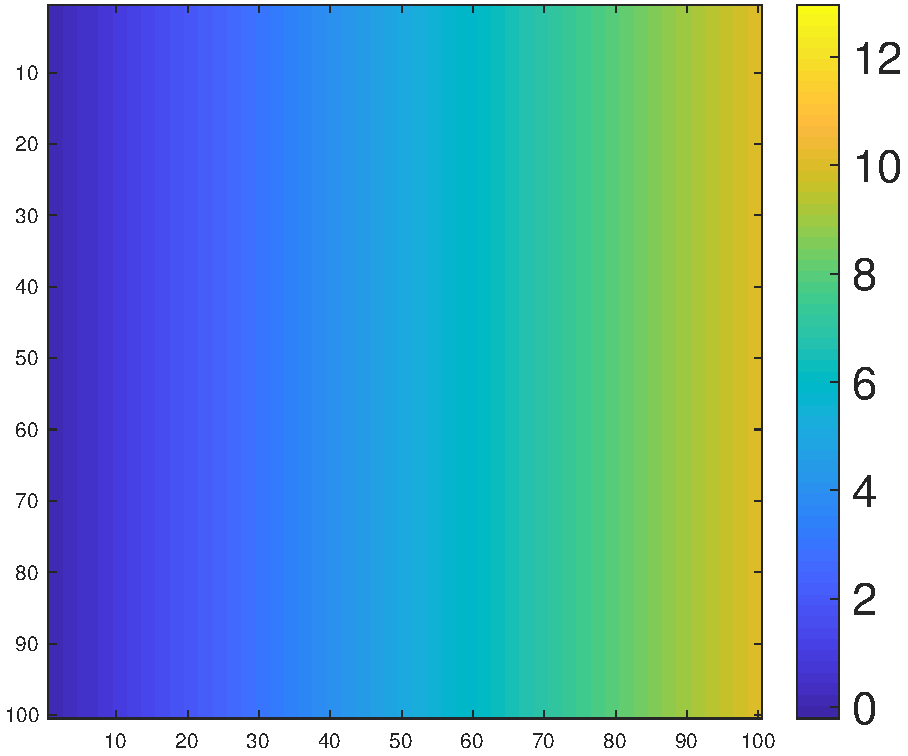
\includegraphics[height=2in]{CIC_linear_ramp_example.pdf}\label{fig:linear_ramp_true}}

  \subfigure[The sample mean field $\bar{X}(\bm{s})$]{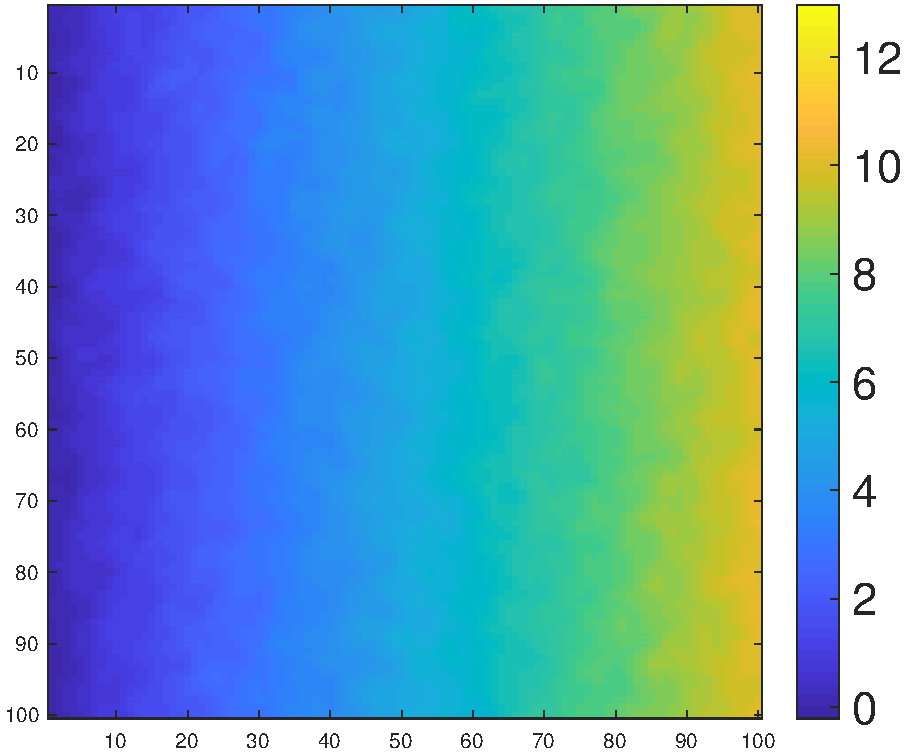
\includegraphics[height=2in]{CIC_linear_ramp_sample_mean.pdf}\label{fig:linear_ramp_sample_mean}}\hspace{1em}
  \subfigure[The sample Cohen's $d$ field $\hat{d}(\bm{s}) = \frac{\bar{X}(\bm{s})}{\hat{\sigma}(\bm{s})}$]{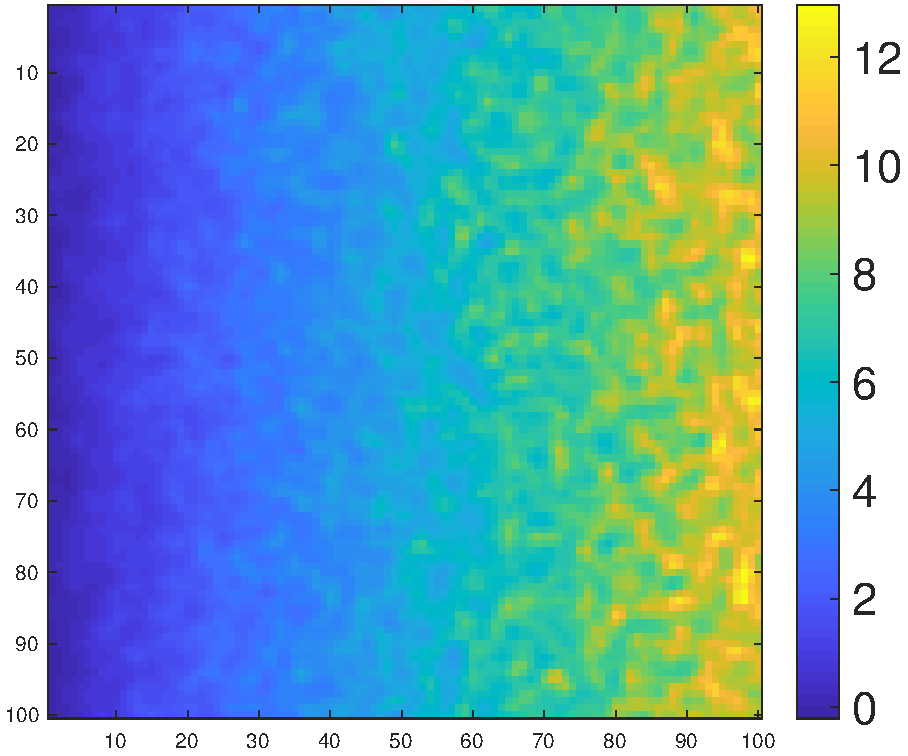
\includegraphics[height=2in]{CIC_linear_ramp_sample_cohen_d.pdf}\label{fig:linear_ramp_cohen_d}}
  \caption{Visualizing the differences between the sample mean and sample Cohen's $d$ field from the 2D simulation. While the sample mean image appears to be uniformly smooth across the region, the sample Cohen's $d$ field becomes rougher from left-to-right.}
\label{fig:visual_example}
\end{figure}

In Fig.\ \ref{fig:linear_ramp_sample_mean} and Fig.\ \ref{fig:linear_ramp_cohen_d} we show the sample mean and sample Cohen's $d$ fields from this simulation. While the sample mean image is uniformly smooth across the space, the Cohen's $d$ field becomes more speckled from left-to-right. Comparing the sample fields with the true underlying signal, readings in each column of the sample mean image appear to be evenly centred around the true underlying effect size. This is not the case for the estimated Cohen's $d$ image, where looking at the far-right column, an appreciable quantity of values are close to 12 when the true underlying effect size was 10. Altogether, this suggests that the moments of the sample Cohen's $d$ may be dependent on the true underlying effect size. In the following section we will derive the limiting properties of the Cohen's $d$ estimator for Gaussian data, before proposing our theoretical adjustments to the method presented in Chapter \ref{chap:BOLD} to obtain CSs for Cohen's $d$ effect size images. 

\subsection{Limiting Properties of the Cohen's d Estimator}
\label{sec:gauss_sig_plus_noise}
Motivated by the example in Fig.\ \ref{fig:visual_example}, we now consider the one-sample model
\begin{equation}
\label{eq:sig_plus_noise}
Y_{i}(\bm{s}) = \mu(\bm{s}) + \epsilon_{i}(\bm{s}), \qquad i = 1, ..., N
\end{equation}
for i.i.d. Gaussian data $Y_{1}(\bm{s}), ..., Y_{N}(\bm{s}) \sim \mathcal{N}(\mu(\bm{s}),\sigma^{2}(\bm{s}))$, with sample mean and standard deviation:
\begin{equation}
\label{eq:unbiased_estimators}
\bar{X}(\bm{s}) = \frac{1}{N}\sum_{i=1}^{N} Y_{i}(\bm{s}), \hspace{10pt} \sigmahat^{2}(\bm{s}) = \frac{1}{N}\sum_{i=1}^{N} \Big(Y_{i}(\bm{s}) - \bar{X}(\bm{s})\Big)^{2}.    
\end{equation}

We wish to understand the limiting structure of the Cohen's $d$ estimator $\hat{d}(\bm{s}) = \frac{\bar{X}(\bm{s})}{\hat{\sigma}(\bm{s})}$. Applying the multivariate central limit theorem, $\bar{X}(\bm{s})$ and $\hat{\sigma}(\bm{s})$ have joint limiting distribution: 
\begin{equation}
\label{eq:joint_limiting_distribution}
\sqrt{N}\Big(\Big(\bar{X}(\bm{s}), \hat{\sigma}(\bm{s})\Big) - \Big(\mu(\bm{s}),\sigma(\bm{s})\Big)\Big) \rightarrow \mathcal{N}\Big(0, \Sigma(\bm{s}) \Big),
\end{equation}
where
\begin{equation}
\label{eq:covariance_matrix}
\Sigma(\bm{s}) = \begin{pmatrix}
			\sigma^{2}(\bm{s}) & 0 \\
            0 & \frac{\sigma^{2}(\bm{s})}{2} 
         \end{pmatrix}.
\end{equation}
Applying the multivariate delta method to (\ref{eq:joint_limiting_distribution}) with the function $f(x,y) = \frac{x}{\sqrt{y}}$, this yields:
\begin{equation}
\label{eq:cohen_limiting_distribution}
\sqrt{N}\Bigg( \frac{\bar{X}(\bm{s})}{\hat{\sigma}(\bm{s})} - \frac{\mu(\bm{s})}{\sigma(\bm{s})} \Bigg) \rightarrow \mathcal{N}\Bigg(0, 1 + \frac{\mu^{2}(\bm{s})}{2\sigma^{2}(\bm{s})} \Bigg).
\end{equation}
Therefore, the limiting field of the Cohen's $d$ estimator $\hat{d}(\bm{s})$ is asymptotically normal with asymptotic variance $1 + \frac{d^{2}(\bm{s})}{2}$. As alluded to in the previous section, it is notable that unlike the sample mean, the asymptotic variance of the Cohen's $d$ estimator is dependent on the underlying true effect size.

We will now assume that the errors are i.i.d. $\epsilon_{1}(\bm{s}), ..., \epsilon_{N}(\bm{s}) \sim \epsilon(\bm{s})$, where $\epsilon(\bm{s})$ is a mean zero Gaussian random field such that for all $\bm{s}, \bm{t} \in S$:
\begin{equation}
\label{eq:covariance_of_errors}
\Cov[\epsilon(\bm{s}),\epsilon(\bm{t})] = \sigma(\bm{s})\sigma(\bm{t})\rho(\bm{s},\bm{t}),
\end{equation}
where $\rho(\bm{s},\bm{t})$ is the Pearson correlation coefficient. In this case, we can also derive the covariance of the limiting distribution. Consider the vector:

\begin{equation}
\label{eq:16}
\begin{pmatrix}
	Y_i(\bm{s}) \\
    (Y_i(\bm{s}) - \mu(\bm{s}))^{2} \\
    Y_i(\bm{t}) \\
    (Y_i(\bm{t}) - \mu(\bm{t}))^{2} 
\end{pmatrix}
\end{equation}
which has mean $\Big(\mu(\bm{s}),\epsilon^{2}(\bm{s}),\mu(\bm{t}),\epsilon^{2}(\bm{t})\Big)$ and covariance matrix:

\begin{equation}
\label{eq:17}
\Sigma(\bm{s},\bm{t}) = 
\begin{pmatrix}
	\sigma^{2}(\bm{s}) & 0 & \sigma(\bm{s})\sigma(\bm{t})\rho(\bm{s},\bm{t}) & 0  \\
    0 & 2\sigma^{4}(\bm{s}) & 0 & 2\sigma^{2}(\bm{s})\sigma(\bm{t})^{2}\rho^{2}(\bm{s},\bm{t}) \\
    \sigma(\bm{s})\sigma(\bm{t})\rho(\bm{s},\bm{t}) & 0 & \sigma^{2}(\bm{t}) & 0 \\
   0 & 2\sigma^{2}(\bm{s})\sigma^{2}(\bm{t})\rho^{2}(\bm{s},\bm{t}) & 0 & 2\sigma^{4}(\bm{t})
\end{pmatrix}
\end{equation}
By implementing the multivariate central limit theorem once again, from above we deduce the asymptotic joint distribution:
\begin{equation}
\label{eq:joint_limiting_distribution_again}
\sqrt{N}\Big(\Big(\bar{X}(\bm{s}), \hat{\sigma}^{2}(\bm{s}), \bar{X}(\bm{t}), \hat{\sigma}^{2}(\bm{t}) \Big) - \Big(\mu(\bm{s}),\sigma^{2}(\bm{s}),\mu(\bm{t}),\sigma^{2}(\bm{t})\Big)\Big) \rightarrow \mathcal{N}\Big(0, \Sigma(\bm{s},\bm{t}) \Big).
\end{equation}
Applying the multivariate delta method with the function $g(x_{1}, y_{1}, x_{2}, y_{2}) = \Big( \frac{x_{1}}{\sqrt{y_1}}, \frac{x_{2}}{\sqrt{y_{2}}} \Big)$ yields:
\begin{equation}
\label{eq:cohen_limiting_distribtuion_covariance}
\sqrt{N}\Bigg( \Bigg(\frac{\bar{X}(\bm{s})}{\hat{\sigma}(\bm{s})}, \frac{\bar{X}(\bm{t})}{\hat{\sigma}(\bm{t})} \Bigg) - \Bigg(\frac{\mu(\bm{s})}{\sigma(\bm{s})}, \frac{\mu(\bm{t})}{\sigma(\bm{t})} \Bigg) \Bigg) \rightarrow \mathcal{N}\Big(0, \Sigma^{*}(\bm{s},\bm{t}) \Big),
\end{equation}
where:
\begin{equation}
\label{eq:cohen_limiting_covariance_matrix}
 \Sigma^{*}(\bm{s},\bm{t}) = \begin{pmatrix}
	1 + \frac{d^{2}({\bm{s}})}{2} & \rho(\bm{s},\bm{t}) + \rho^{2}(\bm{s},\bm{t})\frac{d({\bm{s}})d({\bm{t}})}{2} \\
    \rho(\bm{s},\bm{t}) + \rho^{2}(\bm{s},\bm{t})\frac{d({\bm{s}})d({\bm{t}})}{2} & 1 + \frac{d^{2}({\bm{t}})}{2}
\end{pmatrix}.
\end{equation}

\subsection{Spatial Confidence Sets for Cohen's d Effect Size Images}
\label{sec:confidence_sets_for_cohens_d}
Once again, consider the model outlined at the start of Section {\ref{sec:BOLD_to_cohen}}. For clarity, we reiterate that the spatial CSs for the raw \%BOLD change field $\mu(\bm{s})$ of focus in our previous work took the form:
\begin{equation}
\label{eq:mu_CSs_again}
\Ahatcpmu := \Bigg\{\bm{s} : \bar{X}(\bm{s}) \geq c + \frac{k}{\sqrt{N}}\, \hat{\sigma}(\bm{s}) \Bigg\}, \quad \Ahatcmmu := \Bigg\{\bm{s} : \bar{X}(\bm{s}) \geq c - \frac{k}{\sqrt{N}} \,\hat{\sigma}(\bm{s})  \Bigg\},
\end{equation}
where $k$ was determined via a Wild $t$-bootstrap procedure. Such a construction of the CSs was motivated by the limiting properties of the field:
\begin{equation}
\label{eq:percent_BOLD_normalised error_field}
M(\bm{s}) = \sqrt{N} \cdot \frac{\bar{X}(\bm{s}) - \mu(\bm{s})}{\hat{\sigma}(\bm{s})}.
\end{equation}
In particular, letting $\dAcmu$ denote the boundary of $\Acmu$ defined in (\ref{eq:mu_excursion}), then on a neighbourhood $U$ of $\dAcmu$, it was shown in \textit{SSS} that $M(\bm{s})$ converges weakly to a smooth Gaussian field $G(\bm{s})$ on $U$ with mean zero, unit variance, and with the same (unknown) spatial correlation as each of the $\epsilon_{i}$. 

In the previous section, for the model given in (\ref{eq:sig_plus_noise}) we derived the pointwise convergence of the function:
\begin{equation}
\label{eq:Cohens_d_normalised error_field}
N(\bm{s}) = \sqrt{N} \cdot \frac{\hat{d}(\bm{s}) - d(\bm{s})}{\sqrt{1 + \frac{d^{2}({\bm{s}})}{2}}}
\end{equation}
to a Gaussian field $\mathcal{G}(\bm{s})$ with mean zero, unit variance, and covariance structure:
\begin{equation}
\label{eq:limiting_covariance_structure}
\Cov[\mathcal{G}(\bm{s}),\mathcal{G}(\bm{t})] = \frac{\rho(\bm{s},\bm{t}) + \rho(\bm{s},\bm{t})^{2}\frac{d({\bm{s}})d({\bm{t}})}{2}}{\sqrt{\Big(1 + \frac{d({\bm{s}})^{2}}{2}\Big)\Big(1 + \frac{d({\bm{t}})^{2}}{2}\Big)}}.
\end{equation}
This suggests a natural analog to the construction of CSs in (\ref{eq:mu_CSs_again}) for the Cohen's $d$ effect size given by: 
\begin{equation}
\label{eq:cohens_CSs}
\Ahatcpd := \Bigg\{\bm{s} : \hat{d}(\bm{s}) \geq c + \frac{k}{{\sqrt{N}}}\, \sqrt{1 + \frac{\hat{d}^{2}({\bm{s}})}{2}}\Bigg\}, \quad \Ahatcmd := \Bigg\{\bm{s} : \hat{d}(\bm{s}) \geq c - \frac{k}{{\sqrt{N}}} \,\sqrt{1 + \frac{\hat{d}^{2}({\bm{s}})}{2}}  \Bigg\}.
\end{equation}
Ideally, we wish to apply the same Wild $t$-bootstrap procedure described in Section \ref{sec:wild_bootstrap} of Chapter \ref{chap:BOLD} to approximate the limiting field $G(\bm{s})$ in order to determine $k$. However, we will now show that such an approach is not viable for Cohen's $d$, before proposing a modified procedure to solve the problem. Going forward our focus will mainly be on the Cohen's $d$ effect size, and thus for brevity, we will drop the subscript from our notation and refer to the Cohen's $d$ CSs above as $\Ahatcp$ and $\Ahatcm$ respectively.


\subsection{Modified Residuals for the Cohen's d Wild t-bootstrap}
\label{sec:Wild_t_bootstrap}
In \textit{SSS}, it was shown that the limiting coverage of the CSs for the \%BOLD effect size $\mu(\bm{s})$ is governed by the maximum distribution of the limiting Gaussian field $G(\bm{s})$ on the boundary $\dAcmu$ such that:
\begin{equation}
\label{Result_1}
\lim_{n\rightarrow\infty} P  \Bigg[\Ahatcpmu \subset \Acmu \subset \Ahatcmmu \Bigg] = P \Bigg[\sup_{\bm{s}\in\dAcmu}|G(\bm{s})|\leq k\Bigg].
\end{equation}
Since the limiting Gaussian field $G(\bm{s})$ is unknown, in Chapter \ref{chap:BOLD} we implemented a Wild $t$-bootstrap procedure to approximate $G(\bm{s})$ on the boundary $\dAcmu$. Defining the standardized residuals:
\begin{equation}
\label{eq:standardized_residuals}
\tilde{\epsilon}_{i}(\bm{s}) = \frac{ Y_{i}(\bm{s}) - \bar{X}(\bm{s})}{\hat{\sigma}(\bm{s})},
\end{equation}
then the Wild $t$-bootstrap approximating field is given by:
\begin{equation}
\label{eq:wild_bootstrap_approximating_field}
\tilde{G}^{*}(\bm{s}) = \frac{1}{\sqrt{N}}\sum_{i=1}^{N} r^*_i\frac{\tilde{\epsilon}_{i}(\bm{s})}{\hat{\sigma}^*(\bm{s})},
\end{equation}
where the $r^{*}_i$ are i.i.d.\ Rademacher variables, and $\hat{\sigma}^{*}(\bm{s})$ is the standard deviation of the current realization of bootstrapped residuals $r^{*}_i\tilde{\epsilon}_{i}(\bm{s})$. The asterisk ($*$) indicates that $\tilde{G}^{*}(\bm{s})$ is one of many bootstrap samples; in practice, we would obtain a large number $B$ of bootstrap samples $\tilde{G}^{*}(\bm{s})$, and approximate $k$ as the $(1 - \alpha)100$ percentile of the $B$ suprema $\sup_{\bm{s}\in\dAc}|\tilde{G}^*(\bm{s})|$.

While this method is valid in regards to \%BOLD change, for Cohen's $d$ we demonstrate that asymptotically the correlation structure of the approximating field $\tilde{G}^*(\bm{s})$ is incorrect. Consider again the Gaussian model in Section \ref{sec:gauss_sig_plus_noise}. In this instance, the covariance of the approximating field is:
\begin{alignat}{4}
\label{eq:approximate_limiting_covariance_structure}
&&\Cov[\tilde{G}^{*}(\bm{s}),\tilde{G}^{*}(\bm{t})]
&= \frac{1}{N} \sum_{i,j=1}^{N} \frac{\tilde{\epsilon}_{i}(\bm{s})\tilde{\epsilon}_{j}(\bm{t})}{\hat{\sigma}^{*}(\bm{s})\hat{\sigma}^{*}(\bm{t})}\Cov[r_i,r_j] \notag\\
&
&
&= \frac{1}{N} \cdot \frac{1}{\hat{\sigma}^{*}(\bm{s})\hat{\sigma}^{*}(\bm{t})}\cdot\frac{1}{\hat{\sigma}(\bm{s})\hat{\sigma}(\bm{t})} \sum_{i=1}^{N}(Y_i(\bm{s}) - \bar{X}(\bm{s}))(Y_i(\bm{t}) - \bar{X}(\bm{t})) \notag\\
&
&
&\rightarrow \rho(\bm{s},\bm{t}),
\end{alignat}
where we note that since the standardized residuals $\tilde{\epsilon}_{i}(\bm{s})$ are asymptotically Gaussian with unit variance, the bootstrap estimate of the standard deviation of the standardized residuals $\hat{\sigma}^{*}(\bm{s})$ also converges pointwise to 1. Comparing this with the correlation structure of the true limiting field $\mathcal{G}(\bm{s})$ given in (\ref{eq:limiting_covariance_structure}), letting $d(\bm{s}) = d(\bm{t})$ and setting $q = \frac{d^{2}(\bm{s})}{2} \geq 0$, we observe that:
\begin{equation}
\label{eq:wrong_covariance}
\Cov[\mathcal{G}(\bm{s}),\mathcal{G}(\bm{t})] = \frac{\rho(\bm{s},\bm{t}) + \rho^{2}(\bm{s},\bm{t})\frac{d({\bm{s}})d({\bm{t}})}{2}}{\sqrt{\Big(1 + \frac{d^{2}({\bm{s}})}{2}\Big)\Big(1 + \frac{d^{2}({\bm{t}})}{2}\Big)}} = \rho(\bm{s},\bm{t}) \frac{1 + \rho(\bm{s},\bm{t})q}{1 + q} \leq \rho(\bm{s},\bm{t}).
\end{equation}
Therefore, the limiting covariance of the approximating field \textit{overestimates} the covariance function of $\mathcal{G}(\bm{s})$. 

To solve this, we implement a Taylor expansion transformation recently proposed in \textit{FABIAN's PAPER} to construct modified residuals with the desired limiting properties. Motivated by the delta method procedures used in Section \ref{sec:gauss_sig_plus_noise}, an estimation of the residual field for a single subject $i$ is given by:
\begin{equation}
\label{eq:single_subject_residuals}
\mathcal{E}_{i}(\bm{s}) = \frac{Y_{i}(\bm{s})}{Y_{i}(\bm{s}) - \hat{\mu}(\bm{s})} - \frac{\hat{\mu}(\bm{s})}{\hat{\sigma}(\bm{s})} = f\Big(Y_{i}(\bm{s}),(Y_{i}(\bm{s}) - \hat{\mu}(\bm{s}))^{2}\Big) - f\Big(\hat{\mu}(\bm{s}), \hat{\sigma}^{2}(\bm{s})\Big),
\end{equation}
where the function $f(x,y) = \frac{x}{\sqrt{y}}$. A first-order Taylor expansion of $f(x,y)$ about the point $(\hat{\mu}(\bm{s}), \hat{\sigma}^{2}(\bm{s}))$ yields the approximating Cohen's $d$ residuals:
\begin{alignat}{4}
\label{eq:approximating_residuals}
&&R_{i}(\bm{s})
&= \nabla f(\hat{\mu}(\bm{s}),\hat{\sigma}^{2}(\bm{s}))\Bigg( \Big(Y_{i}(\bm{s}),(Y_{i}(\bm{s}) - \hat{\mu}(\bm{s}))^{2}\Big) - \Big(\hat{\mu}(\bm{s}), \hat{\sigma}^{2}(\bm{s}) \Big) \Bigg)^{\intercal}\notag\\
&
&
&= \frac{Y_{i}(\bm{s}) - \hat{\mu}(\bm{s})}{\hat{\sigma}(\bm{s})} - \frac{\hat{\mu}(\bm{s})}{2\hat{\sigma}(\bm{s})}\Bigg( \frac{\big(Y_{i}(\bm{s}) - \hat{\mu}(\bm{s})\big)^{2}}{\hat{\sigma}^{2}(\bm{s})} - 1 \Bigg).
\end{alignat}
Normalizing by the estimated standard deviation of the limiting field $\mathcal{G}(\bm{s})$, we obtain the modified standardized residuals:
\begin{equation}
\label{eq:cohens_d_residuals}
\tilde{R}_{i}(\bm{s}) = \frac{R_{i}(\bm{s})}{\sqrt{1 + \frac{\hat{d}^{2}(\bm{s})}{2}}}.
\end{equation}
In \textit{FABIAN's PAPER}, they prove that the limiting covariance of $\tilde{R}_{i}(\bm{s})$ is equal to the covariance function of $\mathcal{G}(\bm{s})$. Therefore, a modification of (\ref{eq:wild_bootstrap_approximating_field}) leads us to the Cohen's  $d$ version of the Wild $t$-bootstrap approximating field:
\begin{equation}
\label{eq:cohen_d_wild_bootstrap_approximating_field}
\tilde{G}^{*}(\bm{s}) = \frac{1}{\sqrt{N}}\sum_{i=1}^{N} r^*_i\frac{\tilde{R}_{i}(\bm{s})}{\hat{\sigma}^*(\bm{s})},
\end{equation}
where now $\hat{\sigma}^*(\bm{s})$ is the standard deviation of the bootstrapped Cohen's $d$ residuals $r_i^{*}\tilde{R}_{i}(\bm{s})$.

While normalization of the $R_{i}(\bm{s})$ by an estimator of the standard deviation of $\mathcal{G}(\bm{s})$ provides us with residuals that have the correct limiting properties, for application to fMRI data we are compelled to optimize the performance of the method for smaller sample sizes. In this regard, it may be preferable to standardize the $R_i(\bm{s})$ using an estimator tailored to the sample. Noting that the sample mean of the approximating residuals, $\bar{X}_{R}(\bm{s}) = \frac{1}{N} \sum_{i=1}^{N} R_{i}(\bm{s})$, is equal to zero for all $N$, letting:  

\begin{equation}
\label{eq:sd_of_approximate_residuals}
\hat{\sigma}_{R}^{2}(\bm{s}) = \frac{1}{N} \sum_{i=1}^{N} R_{i}^{2}(\bm{s}),
\end{equation}
then an alternative to (\ref{eq:cohens_d_residuals}) is to normalize the Cohen's $d$ residuals by their sample standard deviation so that:
\begin{equation}
\label{eq:alternate_cohens_d_residuals}
\tilde{R}_{i}(\bm{s}) = \frac{R_{i}(\bm{s})}{\hat{\sigma}_{R}(\bm{s})}.
\end{equation}
These standardized residuals could then be used for the Wild $t$-bootstrap approximating field given in (\ref{eq:cohen_d_wild_bootstrap_approximating_field}). In this case, the sample standard deviation should also be accounted for in the formation of the CSs, suggesting an alternate construction to (\ref{eq:cohens_CSs}) given by:
\begin{equation}
\label{eq:alternate_cohens_CSs}
\Ahatcp := \Bigg\{\bm{s} : \hat{d}(\bm{s}) \geq c + \frac{k}{\sqrt{N}}\, \hat{\sigma}_{R}(\bm{s}) \Bigg\}, \quad \Ahatcm := \Bigg\{\bm{s} : \hat{d}(\bm{s}) \geq c - \frac{k}{\sqrt{N}} \,\hat{\sigma}_{R}(\bm{s}) \Bigg\}.
\end{equation}
In Section \textbf{SIMULATIONS SECTION}, we assess the performance of the CSs on synthetic data when the residuals are standardized using either the estimated limiting variance $\sqrt{1 + \frac{\hat{d}^{2}(\bm{s})}{2}}$ or the sample standard deviation $\hat{\sigma}_{R}(\bm{s})$.

\subsection{Finite Properties of the Cohen's d Estimator and a Variance-stabilizing Transformation}
\label{sec:normalizing_cohens_d}
Up to now, we have used the limiting properties of the Cohen's $d$ estimator to motivate two possible constructions for Cohen's $d$ CSs ((\ref{eq:cohens_CSs}) and (\ref{eq:alternate_cohens_CSs})). In this section, we will draw our attention to the distributional properties of $\hat{d}(\bm{s})$ for finite samples to make further improvements on these methods, as well as develop another novel procedure for obtaining CSs based on Gaussianizing the distibution of $\hat{d}(\bm{s})$. 

Again, assuming the Gaussian model described in Section \ref{sec:gauss_sig_plus_noise}, we observe that the Cohen's $d$ estimator can be expressed in the form: 
\begin{equation}
\label{eq:cohens_d_estimator}
\hat{d} = \frac{\bar{X}}{\hat{\sigma}} =  \frac{1}{\sqrt{N}} \cdot \frac{\bar{X}}{\hat{\sigma}/\sqrt{N}} = \frac{1}{\sqrt{N}} \cdot \frac{\frac{\bar{X} - \mu}{\sigma / \sqrt{N}} + \frac{\mu}{\sigma / \sqrt{N}}}{\sqrt{\left(\frac{\hat{\sigma}^{2}}{\sigma^{2}/(N-1)}\right)/(N-1)}}.
\end{equation}
Since $\frac{\bar{X} - \mu}{\sigma / \sqrt{N}}$ is normally distributed with unit variance and zero mean, and $\frac{\hat{\sigma}^{2}}{\sigma^{2}/(N-1)}$ follows a chi-square distribution with $N-1$ degrees of freedom, from the RHS of the equality we see that $\sqrt{N}\hat{d}$ is characterized by a noncentral $t$-distribution with noncentrality parameter $\sqrt{N}d$ and $N - 1$ degrees of freedom. It is known that the noncentral $t$ is asymmetric unless $\mu = 0$; in general, the size of the asymmetry scales with the magnitude of the noncentrality parameter and is inversely proportional to the degrees of freedom. Therefore, we expect the distribution of the Cohen's $d$ estimator to be highly skew when the true effect size is large and the sample size is small. This conflicts with the symmetric construction of the upper and lower CSs $\Ahatcp$ and $\Ahatcm$ given in (\ref{eq:cohens_CSs}) and (\ref{eq:alternate_cohens_CSs}), suggesting that the coverage performance of these two methods may decline in such situations. 

To account for skewness, we adapt a method originally proposed in \textit{\citet*{Laubscher1960-px}} to stabilize the variance of the noncentral $t$, transforming to a distribution which is approximately Gaussian, and hence, symmetric.
\newtheorem{cohen_theorem}{Theorem}
\begin{cohen_theorem} 
\label{thm:Theorem_1}
Assume the one-sample Gaussian model described in Section \ref{sec:gauss_sig_plus_noise}. For fixed $N$, let: $$a = \sqrt{\frac{N-1}{N-3}}, \qquad b = \sqrt{\frac{8N^{2}-17N + 11}{(N-3)(4N-5)^{2}}},$$
and define $$\alpha = \frac{1}{b}, \qquad \beta = \frac{a}{b}.$$
Then for $b^{*}=\sqrt{N}b, \alpha^{*}=\frac{\alpha}{\sqrt{N}},$ and $\beta^{*}=\sqrt{N}\beta$, define the transformation $f : \mathbb{R} \rightarrow \mathbb{R}$ as:
\begin{multline}
    f\Big(\hat{d}\Big) = \sqrt{N} \Bigg[\alpha^{*} \arcsinh\bigg({\beta^{*} \hat{d}}\bigg) - \alpha^{*} \arcsinh\Bigg({\beta^{*} d} \bigg(1 - \frac{3}{4N - 5}\bigg)^{-1} \Bigg) \\
                + \frac{1}{2N}b^{*2}\Bigg(d \bigg(1 - \frac{3}{4N - 5}\bigg)^{-1} \Bigg)\Bigg(\frac{N-1}{N-3} + N d^{2} \bigg(\frac{8N^{2} - 17N + 11}{16(N-3)(N-2)^{2}} \bigg)\Bigg)^{-\frac{1}{2}} \Bigg].
\end{multline}
Then the random variable $f\Big(\hat{d}\Big)$ has, approximately, zero mean and unit variance.  
\end{cohen_theorem}

\begin{proof}
We closely follow the workings given in the `\textbf{2.\ Noncentral \textit{t}.}'\ section of \textit{\citet*{Laubscher1960-px}}. We have shown that $\sqrt{N}\hat{d}$ is distributed by a noncentral $t$-distribution with noncentrality parameter $\sqrt{N}{\hat{d}}$ and $N - 1$ degrees of freedom. Defining:
\begin{equation}
\label{eq:Cn}
C_{N} = \sqrt{\frac{N-1}{2}} \frac{\Gamma\Big(\frac{N-2}{2}\Big)}{\Gamma\Big(\frac{N-1}{2}\Big)},
\end{equation}
where $\Gamma$ is the gamma function, then the expectation and variance of $\sqrt{N}\hat{d}$ are:
\begin{align}
& \E\Big[\sqrt{N}\hat{d}\Big] = \sqrt{N}dC_{N}, \label{eq:cohen_d_expectation}\\
& \mathrm{Var}\Big[\sqrt{N}\hat{d}\Big] =  \frac{N-1}{N-3} + Nd^{2} \Bigg(\frac{N-1}{N-3} - C_{N}^{2} \Bigg). \label{eq:cohen_d_variance}
\end{align}
It is known that $C_{N}$ is well-approximated by the polynomial:
\begin{equation}
\label{eq:Cn_approximation}
C_{N} \approx \Bigg(1 - \frac{3}{4N - 5} \Bigg)^{-1}.
\end{equation}
Substituting into equations (\ref{eq:cohen_d_expectation}) and (\ref{eq:cohen_d_variance}), we deduce approximations of the expectation and variance of $\sqrt{N}\hat{d}$: 
\begin{align}
&  \E\Big[\sqrt{N}\hat{d}\Big] \approx \sqrt{N}d \Bigg(1 - \frac{3}{4N - 5}\Bigg)^{-1} = m_{1}, \label{eq:cohen_d_expectation_approximation}\\
& \mathrm{Var}\Big[\sqrt{N}\hat{d}\Big] \approx  \frac{N-1}{N-3} + N d^{2} \Bigg(\frac{8N^{2} - 17N + 11}{16(N-3)(N-2)^{2}} \Bigg) =  m_{2}. \label{eq:cohen_d_variance_approximation}
\end{align}
Now, noting that: 
\begin{equation}
\label{eq:m1_squared}
m_{1}^{2} = N d^{2} \frac{(4N -5)^{2}}{16(N-2)^{2}},
\end{equation}
then $m_{2}$ can be expressed in the form:
\begin{equation}
\label{eq:m2_alternate_form}
m_{2} = a^{2} + b^{2} m_{1}^{2},
\end{equation}
where $a = \sqrt{\frac{N-1}{N-3}}$, $b = \sqrt{\frac{8N^{2}-17N + 11}{(N-3)(4N-5)^{2}}}$.
Using the variance expression in (\ref{eq:m2_alternate_form}) and applying Corollary 1.\  in \textit{Laubscher}, the approximate variance-stabilizing transformation of $\sqrt{N}\hat{d}$ is given by: 
\begin{alignat}{4}
\label{eq:variance_stabilizing_result}
&&\psi\Big(\sqrt{N}\hat{d}\Big)
&= \int_{0}^{\sqrt{N}\hat{d}} \Big(a^{2} + b^{2} x^{2}\Big)^{-\frac{1}{2}} dx \notag\\
&
&
&=  \alpha \arcsinh\bigg({\beta \sqrt{N} \hat{d}}\bigg),
\end{alignat}
where $\alpha = \frac{1}{b}$ and $\beta = \frac{a}{b}.$ The quadratic Taylor approximation of $\psi\Big(\sqrt{N}\hat{d}\Big)$ about the point $\sqrt{N}\hat{d} =  \E\Big[\sqrt{N}\hat{d}\Big] \approx m_1$ is given by:
\begin{equation}
\label{eq:quadratic taylor approximation}
\psi\Big(\sqrt{N}\hat{d}\Big) \approx \psi(m_{1}) - \frac{1}{2}b^{2}m_{1}m_{2}^{-\frac{1}{2}}.
\end{equation}
Therefore, the random variable:
\begin{equation}
\label{eq:f_d_sqrt_n}
g\Big(\sqrt{N}\hat{d}\Big) = \psi\Big(\sqrt{N}\hat{d}\Big) - \psi(m_{1}) + \frac{1}{2}b^{2}m_{1}m_{2}^{-\frac{1}{2}}        
\end{equation}
will have, approximately, mean zero and unit variance. Substituting the precise expressions for $\psi, m_{1},$ and $m_{2}$  into (\ref{eq:f_d_sqrt_n}) yields:
\begin{multline}
\label{eq:the_root_d_transformation}
    g\Big(\sqrt{N}\hat{d}\Big) = \alpha \arcsinh\bigg({\beta \sqrt{N} \hat{d}}\bigg) - \alpha \arcsinh\Bigg({\beta \sqrt{N} d} \bigg(1 - \frac{3}{4N - 5}\bigg)^{-1} \Bigg) \\
    + \frac{1}{2}b^{2}\Bigg(\sqrt{N}d \bigg(1 - \frac{3}{4N - 5}\bigg)^{-1} \Bigg)\Bigg(\frac{N-1}{N-3} + N d^{2} \bigg(\frac{8N^{2} - 17N + 11}{16(N-3)(N-2)^{2}} \bigg)\Bigg)^{-\frac{1}{2}}.
\end{multline}
At this point, we have established a variance-stabilizing transformation in terms of $\sqrt{N}\hat{d}$, when in practice, we require a transformation in terms of the Cohen's $d$ estimator $\hat{d}$. This is possible by applying a change of variables to $b,\alpha$ and $\beta$. Defining $b^{*} = \sqrt{N}b$, $\alpha^{*} = \frac{1}{b^{*}} = \frac{1}{\sqrt{N}}\alpha$, and $\beta^{*} = \frac{b^{*}}{a} = \sqrt{N}\beta$, substituting into (\ref{eq:the_root_d_transformation}) obtains the desired transformation:
\begin{multline}
\label{eq:the_final_transformation}
    g\Big(\sqrt{N}\hat{d}\Big) := f\Big(\hat{d}\Big) = \sqrt{N} \Bigg[\alpha^{*} \arcsinh\bigg({\beta^{*} \hat{d}}\bigg) - \alpha^{*} \arcsinh\Bigg({\beta^{*} d} \bigg(1 - \frac{3}{4N - 5}\bigg)^{-1} \Bigg) \\
                + \frac{1}{2N}b^{*2}\Bigg(d \bigg(1 - \frac{3}{4N - 5}\bigg)^{-1} \Bigg)\Bigg(\frac{N-1}{N-3} + N d^{2} \bigg(\frac{8N^{2} - 17N + 11}{16(N-3)(N-2)^{2}} \bigg)\Bigg)^{-\frac{1}{2}} \Bigg].
\end{multline}
\end{proof}
Numerical work presented in \textit{\citet*{Laubscher1960-px}} shows that the 90th percentile value of $f\Big(\hat{d}\Big)$ in (\ref{eq:the_final_transformation}) closely estimates $\phi^{-1}({0.9})$ for a range of true effect sizes $d$ when the sample size is larger than 40. This suggests that, for moderate sample sizes, the distribution of $f\Big(\hat{d}\Big)$ is approximately Gaussian.

An immediate observation from the proof of Theorem \ref{thm:Theorem_1}.\ is that the estimated expectation of $\hat{d}$ is: 
\begin{equation}
\label{eq:estimated_expection_of_d_hat}
\E\Big[\hat{d}\Big] \approx d \bigg(1 - \frac{3}{4N - 5}\bigg)^{-1},
\end{equation}
and therefore, unlike the sample mean, the Cohen's $d$ estimator is biased. To improve the performance of the CSs for small sample sizes, this bias should be accounted for in the formulation of the CSs. This leads to a bias-corrected version of the CS construction in (\ref{eq:cohens_CSs}) given by: 
\begin{equation}
\label{eq:bias_corrected_cohens_CSs}
\Ahatcpm := \Bigg\{\bm{s} : \hat{d}(\bm{s}) \geq c\bigg(1 - \frac{3}{4N - 5}\bigg)^{-1} \pm \frac{k}{{\sqrt{N}}}\, \sqrt{1 + \frac{\hat{d}^{2}({\bm{s}})}{2}}\Bigg\}, 
\end{equation}
and similarly, a bias-corrected version of the alternate construction in (\ref{eq:alternate_cohens_CSs}) given by:
\begin{equation}
\label{eq:bias_corrected_alternate_cohens_CSs}
\Ahatcpm := \Bigg\{\bm{s} : \hat{d}(\bm{s}) \geq c\bigg(1 - \frac{3}{4N - 5}\bigg)^{-1} \pm \frac{k}{\sqrt{N}}\, \hat{\sigma}_{R}(\bm{s}) \Bigg\}.
\end{equation}
Additionally, for any application to real data the Wild $t$-Bootstrap described in Section \ref{sec:Wild_t_bootstrap} must be applied over an approximation of the boundary $\dAc = \{\bm{s} \in S : d(\bm{s}) = c \}$. Taking into consideration the bias of the Cohen's $d$ estimator, we will therefore use the plug-in boundary:
\begin{equation}
\label{eq:plug_in_boundary}
\dAhatc = \Bigg\{\bm{s} \in S : \hat{d}(\bm{s}) = c\bigg(1 - \frac{3}{4N - 5}\bigg)^{-1} \Bigg\}.
\end{equation}
Finally, by the monotonicity of the mapping $x \mapsto \alpha^{*} \arcsinh\bigg({\beta^{*} x}\bigg)$, another possibility is to construct the CSs in the transformed domain $f(S)$. From Theorem \ref{thm:Theorem_1}, the transformed CSs are constructed as:
\begin{multline}
\label{eq:transformed_cohens_CSs}
    \Ahatcpm = \Bigg\{\bm{s} : \alpha^{*} \arcsinh\Bigg(\beta^{*} \hat{d}(\bm{s}) \Bigg) \geq \alpha^{*} \arcsinh\Bigg(\beta^{*} c \Bigg(1 - \frac{3}{4N -5}\Bigg)^{-1} \Bigg) \\
    - \frac{1}{2N}b^{*2}\Bigg(c \bigg(1 - \frac{3}{4N - 5}\bigg)^{-1} \Bigg)\Bigg(\frac{N-1}{N-3} + N c^{2} \bigg(\frac{8N^{2} - 17N + 11}{16(N-3)(N-2)^{2}} \bigg)\Bigg)^{-\frac{1}{2}} \pm \frac{k}{\sqrt{N}} \Bigg\}. 
\end{multline}
In this case, the Cohen's $d$ residuals given in (\ref{eq:approximating_residuals}) for the Wild $t$-Bootstrap must also be modified. An estimation of the transformed residual field for a single subject $i$ is given by: 
\begin{alignat}{4}
\label{eq:single_subject_transformed_residuals}
&&\mathcal{E}_{i}(\bm{s})
& = \alpha^{*} \arcsinh\Bigg(\beta^{*} \frac{Y_{i}(\bm{s})}{Y_{i}(\bm{s}) - \hat{\mu}(\bm{s})} \Bigg) - \alpha^{*} \arcsinh\Bigg(\beta^{*} \frac{\hat{\mu}(\bm{s})}{\hat{\sigma}(\bm{s})} \Bigg)\notag\\
&
&
&= h\Big(Y_{i}(\bm{s}),(Y_{i}(\bm{s}) - \hat{\mu}(\bm{s}))^{2}\Big) - h\Big(\hat{\mu}(\bm{s}), \hat{\sigma}^{2}(\bm{s})\Big),
\end{alignat}
%\begin{equation}
%\label{eq:single_subject_transformed_residuals}
%\mathcal{E}_{i}(\bm{s}) = \alpha^{*} \arcsinh\Bigg(\beta^{*} \frac{Y_{i}(\bm{s})}{Y_{i}(\bm{s}) - \hat{\mu}(\bm{s})} \Bigg) - \alpha^{*} \arcsinh\Bigg(\beta^{*} \frac{\hat{\mu}(\bm{s})}{\hat{\sigma}(\bm{s})} \Bigg) = h\Big(Y_{i}(\bm{s}),(Y_{i}(\bm{s}) - \hat{\mu}(\bm{s}))^{2}\Big) - h\Big(\hat{\mu}(\bm{s}), \hat{\sigma}^{2}(\bm{s})\Big),
%\end{equation}
where the function $h(x,y) =  \alpha^{*} \arcsinh\Bigg(\beta^{*} \frac{x}{\sqrt{y}}\Bigg)$. Similarly to the methods applied in Section \ref{sec:Wild_t_bootstrap}, a first-order Taylor expansion of $h(x,y)$ about the point $(\hat{\mu}(\bm{s}), \hat{\sigma}^{2}(\bm{s}))$ obtains the transformed Cohen's $d$ residuals:
\begin{alignat}{4}
\label{eq:transformed_approximating_residuals}
&&\tilde{R}_{i}(\bm{s})
&= \nabla h(\hat{\mu}(\bm{s}),\hat{\sigma}^{2}(\bm{s}))\Bigg( \Big(Y_{i}(\bm{s}),(Y_{i}(\bm{s}) - \hat{\mu}(\bm{s}))^{2}\Big) - \Big(\hat{\mu}(\bm{s}), \hat{\sigma}^{2}(\bm{s}) \Big) \Bigg)^{\intercal}\notag\\
&
&
&= \frac{\alpha^{*}\beta^{*}}{\sqrt{1 + \beta^{*2}\frac{\hat{\mu}^{2}(\bm{s})}{\hat{\sigma}^{2}(\bm{s})}}} \Bigg(\frac{Y_{i}(\bm{s}) - \hat{\mu}(\bm{s})}{\hat{\sigma}(\bm{s})} - \frac{\hat{\mu}(\bm{s})}{2\hat{\sigma}(\bm{s})}\Bigg( \frac{\big(Y_{i}(\bm{s}) - \hat{\mu}(\bm{s})\big)^{2}}{\hat{\sigma}^{2}(\bm{s})} - 1 \Bigg)\Bigg).
\end{alignat}
In practice, the critical value $k$ in (\ref{eq:transformed_cohens_CSs}) is computed by applying the Wild $t$-Bootstrap over $\dAhatc$ using the above transformed Cohen's $d$ residuals for the bootstrap approximating field in (\ref{eq:cohen_d_wild_bootstrap_approximating_field}). 

For coherence, we will now formalize the complete procedures to obtain CSs for each of our three proposed CS constructions in (\ref{eq:bias_corrected_cohens_CSs}), (\ref{eq:bias_corrected_alternate_cohens_CSs}), and (\ref{eq:transformed_cohens_CSs}).

\subsection{Three Algorithms for Computing Cohen's d CSs}
Based on our derivations up to this point, we give three algorithms to compute Cohen's $d$ CSs for data modelled within the one-sample model in Section \ref{sec:BOLD_to_cohen}. While the first two algorithms are similar, the key difference separating these methods is the estimator of the variance used in the formation of the CSs and for standardizing the Cohen's $d$ residuals. We first describe Algorithm \ref{alg:one}, where we use $1 + \frac{\hat{d}^{2}(\bm{s})}{2}$ as the estimator of the variance, motivated by the variance of the limiting field $\mathcal{G}(\bm{s})$ derived in Sections \ref{sec:gauss_sig_plus_noise} and \ref{sec:confidence_sets_for_cohens_d}.

\newtheorem{algorithm}{Algorithm}
\begin{algorithm}
\label{alg:one}
For observations $Y_{1}(\bm{s}), ..., Y_{N}(\bm{s})$ over a spatial domain $S$ following the one-sample linear model in (\ref{eq:Cohen_GLM}), the following procedure yields CSs for the Cohen's $d$ image $\hat{d}(\bm{s}) = \frac{\hat{\mu}(\bm{s})}{\hat{\sigma}(\bm{s})}$ corresponding to a fixed threshold $c$ and confidence level $(1 - \alpha)\%$.
\begin{enumerate}
\item For each observation $Y_i(\bm{s})$ let $\hat{\epsilon}_{i}(\bm{s})$ denote the residual field, $\hat{\epsilon}_{i}(\bm{s}) = Y_{i}(\bm{s}) - \hat{\mu}(\bm{s})$. Then compute the Cohen's $d$ residuals as: 
$$R_{i}(\bm{s}) = \frac{\hat{\epsilon}_{i}(\bm{s})}{\hat{\sigma}(\bm{s})} - \frac{\hat{\mu}(\bm{s})}{2\hat{\sigma}(\bm{s})}\Bigg( \frac{\hat{\epsilon}_{i}^{2}(\bm{s})}{\hat{\sigma}^{2}(\bm{s})} - 1 \Bigg).$$ 
\item Normalize the Cohen's $d$ residuals by the estimated limiting standard deviation of the Cohen's $d$ image to obtain the standardized residuals:
$$\tilde{R}_{i}(\bm{s}) = \frac{R_{i}(\bm{s})}{\sqrt{1 + \frac{\hat{\mu}^{2}(\bm{s})}{2\hat{\sigma}^{2}(\bm{s})}}}.$$ 
\item Draw $N$ i.i.d.\ Rademacher variables $r_{1}^{*}, ..., r_{N}^{*}$, and compute the Wild $t$-Bootstrap approximating field:
$$\tilde{G}^{*}(\bm{s}) = \frac{1}{\sqrt{N}}\sum_{i=1}^{N} r^*_i\frac{\tilde{R}_{i}(\bm{s})}{\hat{\sigma}^*(\bm{s})},$$
where $\hat{\sigma}^{*}(\bm{s})$ is the bootstrap standard deviation of the bootstrapped residuals $r_{i}\tilde{R}_{i}(\bm{s})$. 
\item Obtain the value $k^{*} = \sup_{\bm{s}\in\dAhatc}|G^{*}(\bm{s})|$, using the bias-corrected estimator of the boundary $\dAhatc = \Bigg\{\bm{s} \in S : \hat{d}(\bm{s}) = c\bigg(1 - \frac{3}{4N - 5}\bigg)^{-1} \Bigg\}$.
\item For a large number of bootstrap replications B repeat steps 3.\ and 4., obtaining the empirical distribution of the absolute maximum $\mathcal{K}_{B} = \{k_{1}^{*}, ..., k_{B}^{*}\}$. Compute $k$ as the $(1 - \alpha)$ percentile of $\mathcal{K}_{B}$.
\item Obtain the Cohen's $d$ CSs:
$$\Ahatcpm := \Bigg\{\bm{s} : \hat{d}(\bm{s}) \geq c\bigg(1 - \frac{3}{4N - 5}\bigg)^{-1} \pm \frac{k}{{\sqrt{N}}}\, \sqrt{1 + \frac{\hat{d}^{2}({\bm{s}})}{2}}\Bigg\}.$$
\end{enumerate}
\end{algorithm}

We now describe Algorithm \ref{alg:two}. Here, we use the sample variance of the Cohen's $d$ residuals $\hat{\sigma}_{R}^{2}(\bm{s})$ as the variance estimator, motivated by our workings in Section \ref{sec:Wild_t_bootstrap}.

\begin{algorithm}
\label{alg:two}
For observations $Y_{1}(\bm{s}), ..., Y_{N}(\bm{s})$ over a spatial domain $S$ following the one-sample linear model in (\ref{eq:Cohen_GLM}), the following procedure yields CSs for the Cohen's $d$ image $\hat{d}(\bm{s}) = \frac{\hat{\mu}(\bm{s})}{\hat{\sigma}(\bm{s})}$ corresponding to a fixed threshold $c$ and confidence level $(1 - \alpha)\%$.
\begin{enumerate}
\item For each observation $Y_i(\bm{s})$ let $\hat{\epsilon}_{i}(\bm{s})$ denote the residual field, $\hat{\epsilon}_{i}(\bm{s}) = Y_{i}(\bm{s}) - \hat{\mu}(\bm{s})$. Then compute the Cohen's $d$ residuals as: 
$$R_{i}(\bm{s}) = \frac{\hat{\epsilon}_{i}(\bm{s})}{\hat{\sigma}(\bm{s})} - \frac{\hat{\mu}(\bm{s})}{2\hat{\sigma}(\bm{s})}\Bigg( \frac{\hat{\epsilon}_{i}^{2}(\bm{s})}{\hat{\sigma}^{2}(\bm{s})} - 1 \Bigg).$$ 
\item Normalize the Cohen's $d$ residuals by their sample standard deviation to obtain the standardized residuals:
$$\tilde{R}_{i}(\bm{s}) = \frac{R_{i}(\bm{s})}{\hat{\sigma}_{R}(\bm{s})}.$$ 
\item Draw $N$ i.i.d.\ Rademacher variables $r_{1}^{*}, ..., r_{N}^{*}$, and compute the Wild $t$-Bootstrap approximating field:
$$\tilde{G}^{*}(\bm{s}) = \frac{1}{\sqrt{N}}\sum_{i=1}^{N} r^*_i\frac{\tilde{R}_{i}(\bm{s})}{\hat{\sigma}^*(\bm{s})},$$
where $\hat{\sigma}^{*}(\bm{s})$ is the bootstrap standard deviation of the bootstrapped residuals $r_{i}\tilde{R}_{i}(\bm{s})$. 
\item Obtain the value $k^{*} = \sup_{\bm{s}\in\dAhatc}|G^{*}(\bm{s})|$, using the bias-corrected estimator of the boundary $\dAhatc = \Bigg\{\bm{s} \in S : \hat{d}(\bm{s}) = c\bigg(1 - \frac{3}{4N - 5}\bigg)^{-1} \Bigg\}$.
\item For a large number of bootstrap replications B repeat steps 3.\ and 4., obtaining the empirical distribution of the absolute maximum $\mathcal{K}_{B} = \{k_{1}^{*}, ..., k_{B}^{*}\}$. Compute $k$ as the $(1 - \alpha)$ percentile of $\mathcal{K}_{B}$.
\item Obtain the Cohen's $d$ CSs:
$$\Ahatcpm := \Bigg\{\bm{s} : \hat{d}(\bm{s}) \geq c\bigg(1 - \frac{3}{4N - 5}\bigg)^{-1} \pm \frac{k}{\sqrt{N}}\, \hat{\sigma}_{R}(\bm{s}) \Bigg\}.$$
\end{enumerate}
\end{algorithm}

Finally, we describe Algorithm \ref{alg:three}. Based on the derivations in Section \ref{sec:normalizing_cohens_d}, we transform the estimated Cohen's $d$ image to a field which is approximately Gaussian. This is done to stabilize the variance and remove the skew of the Cohen's $d$ estimator, which may adversely effect the performance of the CSs. By the monotonicity of the transformation, the CSs obtained using this method are valid for inference on the true (un-transformed) Cohen's $d$ effect size. 

\begin{algorithm}
\label{alg:three}
For observations $Y_{1}(\bm{s}), ..., Y_{N}(\bm{s})$ over a spatial domain $S$ following the one-sample linear model in (\ref{eq:Cohen_GLM}), the following procedure yields CSs for the Cohen's $d$ image $\hat{d}(\bm{s}) = \frac{\hat{\mu}(\bm{s})}{\hat{\sigma}(\bm{s})}$ corresponding to a fixed threshold $c$ and confidence level $(1 - \alpha)\%$.
\begin{enumerate}
\item For each observation $Y_i(\bm{s})$ let $\hat{\epsilon}_{i}(\bm{s})$ denote the residual field, $\hat{\epsilon}_{i}(\bm{s}) = Y_{i}(\bm{s}) - \hat{\mu}(\bm{s})$. Then compute the transformed, variance-stabilized Cohen's $d$ residuals as: 
$$\tilde{R}_{i}(\bm{s}) = \frac{\alpha^{*}\beta^{*}}{\sqrt{1 + \beta^{*2}\frac{\hat{\mu}^{2}(\bm{s})}{\hat{\sigma}^{2}(\bm{s})}}} \Bigg(\frac{Y_{i}(\bm{s}) - \hat{\mu}(\bm{s})}{\hat{\sigma}(\bm{s})} - \frac{\hat{\mu}(\bm{s})}{2\hat{\sigma}(\bm{s})}\Bigg( \frac{\big(Y_{i}(\bm{s}) - \hat{\mu}(\bm{s})\big)^{2}}{\hat{\sigma}^{2}(\bm{s})} - 1 \Bigg)\Bigg).$$ 
\item Draw $N$ i.i.d.\ Rademacher variables $r_{1}^{*}, ..., r_{N}^{*}$, and compute the Wild $t$-Bootstrap approximating field:
$$\tilde{G}^{*}(\bm{s}) = \frac{1}{\sqrt{N}}\sum_{i=1}^{N} r^*_i\frac{\tilde{R}_{i}(\bm{s})}{\hat{\sigma}^*(\bm{s})},$$
where $\hat{\sigma}^{*}(\bm{s})$ is the bootstrap standard deviation of the bootstrapped residuals $r_{i}\tilde{R}_{i}(\bm{s})$. 
\item Obtain the value $k^{*} = \sup_{\bm{s}\in\dAhatc}|G^{*}(\bm{s})|$, using the bias-corrected estimator of the boundary $\dAhatc = \Bigg\{\bm{s} \in S : \hat{d}(\bm{s}) = c\bigg(1 - \frac{3}{4N - 5}\bigg)^{-1} \Bigg\}$.
\item For a large number of bootstrap replications B repeat steps 3.\ and 4., obtaining the empirical distribution of the absolute maximum $\mathcal{K}_{B} = \{k_{1}^{*}, ..., k_{B}^{*}\}$. Compute $k$ as the $(1 - \alpha)$ percentile of $\mathcal{K}_{B}$.
\item Obtain the Cohen's $d$ CSs:
\begin{multline}
\label{eq:transformed_cohens_CSs_again}
    \Ahatcpm = \Bigg\{\bm{s} : \alpha^{*} \arcsinh\Bigg(\beta^{*} \hat{d}(\bm{s}) \Bigg) \geq \alpha^{*} \arcsinh\Bigg(\beta^{*} c \Bigg(1 - \frac{3}{4N -5}\Bigg)^{-1} \Bigg) \\
    - \frac{1}{2N}b^{*2}\Bigg(c \bigg(1 - \frac{3}{4N - 5}\bigg)^{-1} \Bigg)\Bigg(\frac{N-1}{N-3} + N c^{2} \bigg(\frac{8N^{2} - 17N + 11}{16(N-3)(N-2)^{2}} \bigg)\Bigg)^{-\frac{1}{2}} \pm \frac{k}{\sqrt{N}} \Bigg\}. 
\end{multline}
\end{enumerate}
\end{algorithm}

\section{Methods}
\subsection{Simulations}
\label{sec:cohen_simulations}
In this section we describe the settings used to evaluate the performance of each of the three algorithms for obtaining Cohen's $d$ CSs on synthetic data. We simulate 3000 independent samples of the Gaussian one-sample model 

$$Y_{i}(\bm{s}) = \mu(\bm{s}) + \epsilon_{i}(\bm{s}), \qquad i = 1, ..., N$$
using a range of signals $\mu(\bm{s})$, Gaussian noise structures $\epsilon_{i}(\bm{s})$ with stationary and non-stationary variance $\sigma^{2}(\bm{s})$, in two- and three-dimensional regions $S$. To compute the critical value $k$, we apply the Wild $t$-Bootstrap method with $B = 5000$ bootstrap samples on the estimated boundary $\dAhatc$ that must be used for applications of the method to real data. We obtain the boundary using the linear interpolation method described in Section \ref{sec:boundary_discrete_lattice} of Chapter \ref{chap:BOLD}. We then compare the empirical coverage -- the percentage of trials that the true thresholded signal is completely contained between the upper and lowers CSs (i.e. the number of times for which $\Ahatcp \subset \Ac \subset \Ahatcm$) -- between the three algorithms, using the interpolation assessment method described in Section \ref{sec:coverage_assessment} of Chapter \ref{chap:BOLD}. In each simulation, we apply the method for sample sizes of $N = 60, 120, 240$ and $480$, and using three nominal coverage probability levels $1 - \alpha = 0.80, 0.90$ and $0.95$. 


\subsection{2D Simulations}
\label{sec:cohen_2D_simulations}
We analyzed the performance of the three algorithms to obtain Cohen's $d$ CSs on a square region of size $100 \times 100$. For the true underlying signal $\mu(\bm{s})$ we considered two different raw effects: First, a linear ramp that increased from a magnitude of 0 to 1 in the $x$-direction while remaining constant in the $y$-direction. Second, a circular effect, created by placing a circular phantom of magnitude 1 and radius 30 in the centre of the search region, which was then smoothed using a 3 voxel FWHM Gaussian kernel. If we were to assume that each voxel had a size of $2$mm$^{3}$, we note that this would amount to applying smoothing with a $6$mm FWHM kernel, a fairly typical setting used in fMRI analyses.

To each of these signals we added subject-specific Gaussian noise $\epsilon_{i}(\bm{s})$, also smoothed using a 3 voxel FWHM Gaussian kernel, with homogeneous and non-homogeneous variance structures: The first noise field had a spatially constant standard deviation of 1, and therefore in this case the true Cohen's $d$ effect was identical to the underlying signal field $\mu(\bm{s})$. The second field had a linearly increasing standard deviation structure in the y-direction from $\sqrt{0.5}$ to $\sqrt{1.5}$ while remaining constant in the x-direction. Thus, the variance of this noise field spatially increased in the y-direction from $0.5$ to $1.5$ in a non-linear fashion. 

\begin{figure}[htbp]
  \centering
  \subfigure[The Cohen's $d$ field $d(\bm{s})$ for the linear ramp signal $\mu(\bm{s})$ and homogeneous noise structure.]{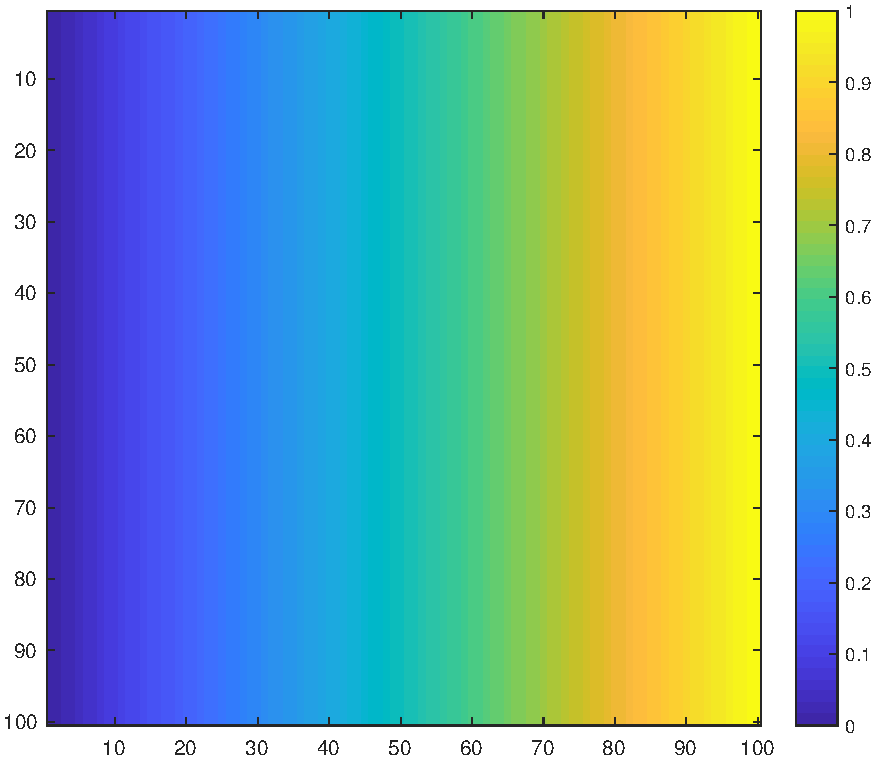
\includegraphics[height=2in]{CIC_linear_ramp_homogeneous_noise.pdf}\label{fig:linear_ramp_homo}}\hspace{1em}
  \subfigure[The Cohen's $d$ field $d(\bm{s})$ for the linear ramp signal $\mu(\bm{s})$ and heterogeneous noise structure.]{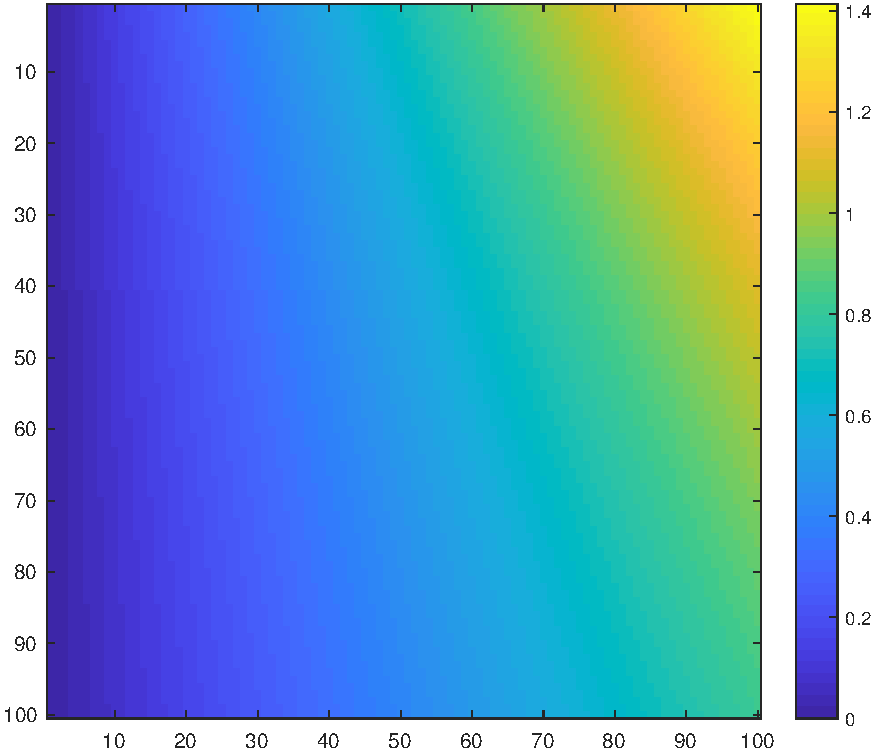
\includegraphics[height=2in]{CIC_linear_ramp_heterogeneous_noise.pdf}\label{fig:linear_ramp_hetero}}
  \caption{The two Cohen's $d$ effects corresponding to the linear ramp signal $\mu(\bm{s})$. On the left, the subject-specific Gaussian noise field $\epsilon_{i}(\bm{s})$ has a spatially constant standard deviation of 1, and therefore $d(\bm{s}) = \mu(\bm{s})$. On the right, $\epsilon_{i}(\bm{s})$ had a spatially increasing standard deviation structure in the y-direction (from top-to-bottom), while remaining constant in the x-direction.} 
\label{fig:linear_ramp_figures}
\end{figure}

\begin{figure}[htbp]
  \centering
  \subfigure[The Cohen's $d$ field $d(\bm{s})$ for the circular signal $\mu(\bm{s})$ and homogeneous noise structure.]{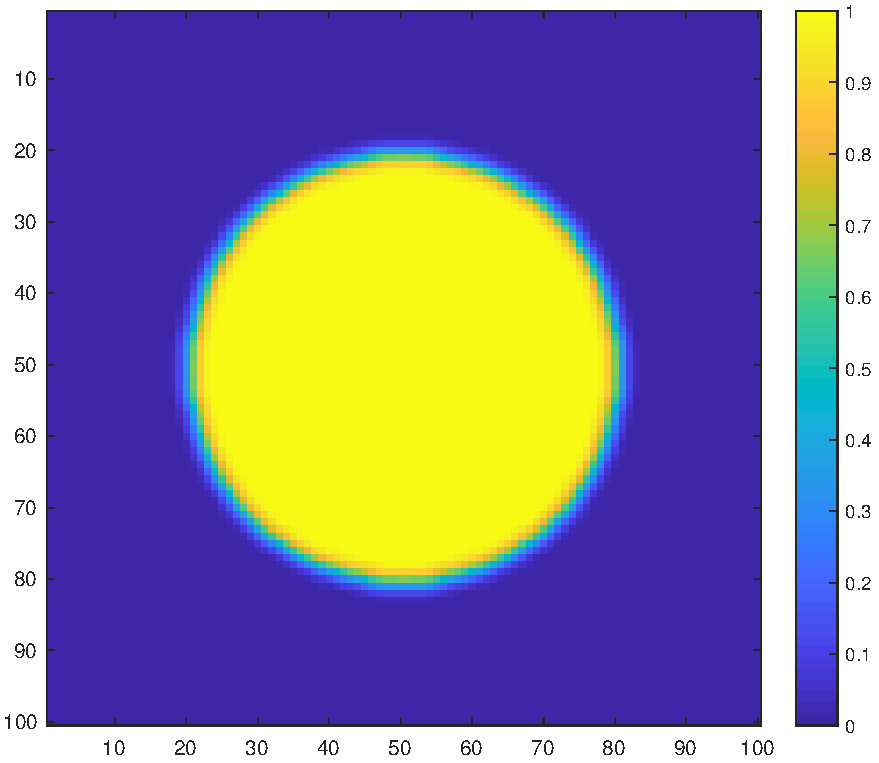
\includegraphics[height=2in]{CIC_circle_homogeneous_noise.pdf}\label{fig:circle_homo}}\hspace{1em}
  \subfigure[The Cohen's $d$ field $d(\bm{s})$ for the circular signal $\mu(\bm{s})$ and heterogeneous noise structure.]{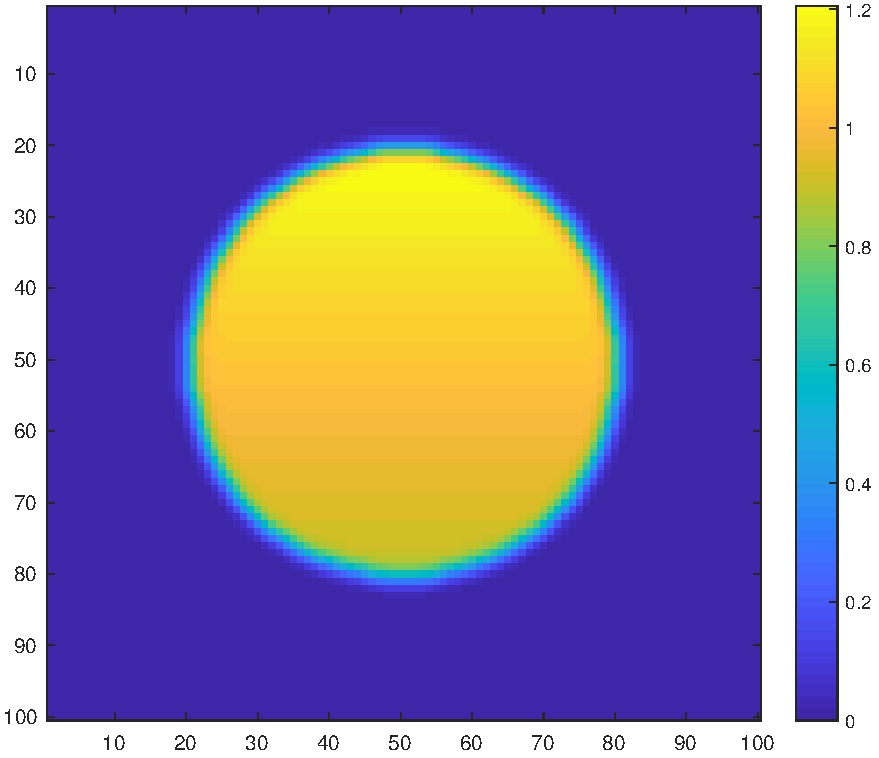
\includegraphics[height=2in]{CIC_circle_heterogeneous_noise.pdf}\label{fig:circle_hetero}}
  \caption{The two Cohen's $d$ effects corresponding to the circular signal $\mu(\bm{s})$. On the left, the subject-specific Gaussian noise field $\epsilon_{i}(\bm{s})$ has a spatially constant standard deviation of 1, and therefore $d(\bm{s}) = \mu(\bm{s})$. On the right, $\epsilon_{i}(\bm{s})$ had a spatially increasing standard deviation structure in the y-direction (from top-to-bottom), while remaining constant in the x-direction.} 
\label{fig:circle_figures}
\end{figure}

The true Cohen's $d$ fields $d(\bm{s})$ for the linear ramp signal with homogeneous and heterogeneous noise are shown in Figure \ref{fig:linear_ramp_figures}. The corresponding Cohen's $d$ fields for the circular signal are shown in Figure \ref{fig:circle_figures}. Altogether, for the three algorithms, the two underlying signals and two noise sources gave us 12 separate trials; across all of the simulations, we obtained Cohen's $d$ Confidence Sets for the noise-free cluster $\Ac$ at a cluster-forming threshold of $c = 0.8$. In Chapter 2.2 of \textit{\citet*{Cohen2013-it}}, $d=0.8$ was classified as a `large effect'; for group-level analyses of large-sample fMRI data with ample statistical power (such as the HCP or UK Biobank), effect sizes of this magnitude would be used to assess brain areas where practically significant (and potentially, clinically important) activation has occurred.



\subsection{3D Simulations}
Four signal types $\mu(\bm{s})$ were considered to analyze the performance of the three algorithms in three dimensions. The first three of these signals were generated synthetically on a cubic region of size $100 \times 100 \times 100$: Firstly, a small spherical effect, created by placing a spherical phantom of magnitude 1 and radius 5 in the centre of the search region, which was then smoothed using a 3 voxel FWHM Gaussian kernel. Secondly, a larger spherical effect, generated identically to the first effect with the exception that the spherical phantom had a radius of 30. Lastly, we created an effect by placing four spherical phantoms of magnitude 1 in the region of varying radii and then smoothing the entire image using a 3 voxel FWHM Gaussian. 

Each of the images were re-scaled after smoothing to have a maximum intensity of 1. For the small and large spherical effect an image-wise re-scaling was applied, where all locations in the smoothed map were divided through by the maximum intensity across the region. For the final effect, because parts of the four spherical phantoms overlapped after smoothing, the signal intensities in these regions summed to greater than 1. In this case, we re-scaled the smoothed map by reducing the intensities in these areas to have a magnitude of 1 while leaving the rest of the image untouched. 

Similar to the two-dimensional simulations, for the three signals described above we added 3-voxel smoothed Gaussian noise with homogeneous and heterogeneous variance structures. The first noise field had a spatially constant standard deviation of 1, while the second field had a linearly increasing standard deviation in the z-direction from $\sqrt{0.5}$ to $\sqrt{1.5}$, while remaining constant in both the x- and y- directions. As demonstrated for the 2D simulations in Figures \ref{fig:linear_ramp_figures} and \ref{fig:circle_figures}, this lead to two different true Cohen's $d$ effect-size images $d(\bm{s})$ corresponding to the homogeneous and heterogeneous standard deviation fields $\sigma(\bm{s})$ used for the noise.

For the final signal type, we took advantage of big data that has been made available through the UK Biobank in an attempt to generate an effect that replicated the true \%BOLD change induced during an fMRI task. We randomly selected 4000 subject-level contrast of parameter estimate result maps from the Hariri Faces/Shapes task-fMRI data collected as part of the UK Biobank brain imaging study. Full details on how the data were acquired and processed is given in \textit{\citet{Miller2016-hd}}, \textit{\citet{Alfaro-Almagro2018-ip}} and the UK Biobank Showcase; information on the task paradigm is given in \textit{\citet{Hariri2002-ns}}. From these contrast maps, we computed a group-level full mean and full standard deviation image. In the final simulation, we used the group-level Biobank mean image as the true underlying signal $\mu(\bm{s})$ for each subject, and the full standard deviation image was used for the standard deviation of each simulated subject-specific Gaussian noise field $\epsilon_{i}(\bm{s})$ added to the true signal. Because of the considerably large sample size of high-quality data from which these maps have been obtained, we anticipate that both of these images are highly representative of the true underlying fields that they approximate. Both images were masked using an intersection of all 4000 of the subject-level brain masks.

\begin{table}[htbp]
\thisfloatpagestyle{empty}
\hspace*{-0.5cm}
\begin{adjustbox}{center}
\centering
    \begin{tabular}{cm{50mm}m{50mm}m{50mm}}
       \toprule
         & \hspace{14.8mm} Z = 50 & \hspace{14.8mm} Z = 60 & \hspace{14.8mm} Z = 70 \\
        \midrule
        (a) Small Sphere & 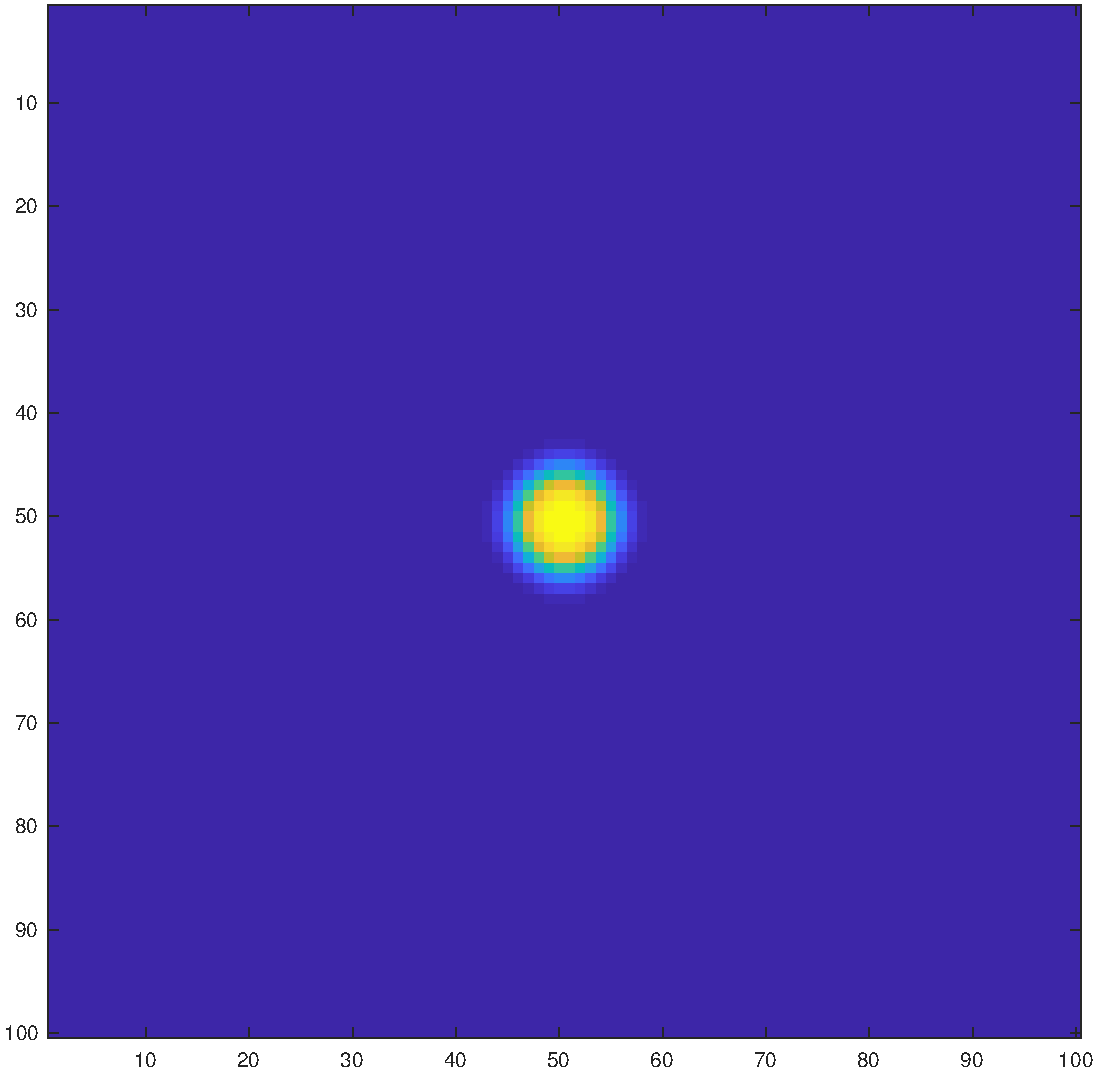
\includegraphics[height=40mm]{CIC_Sig_1_Z50.pdf} & 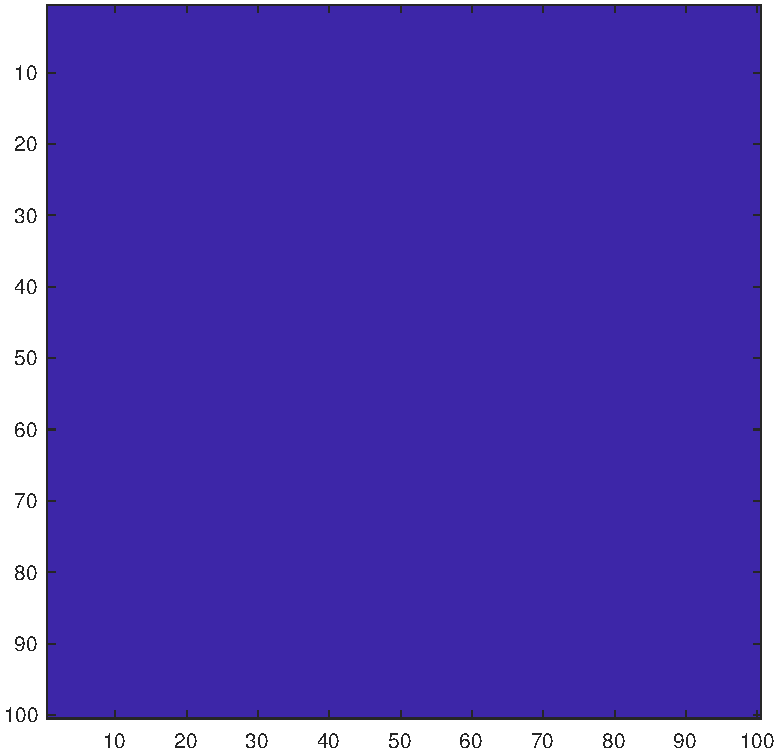
\includegraphics[height=40mm]{CIC_Sig_1_Z60.pdf} & 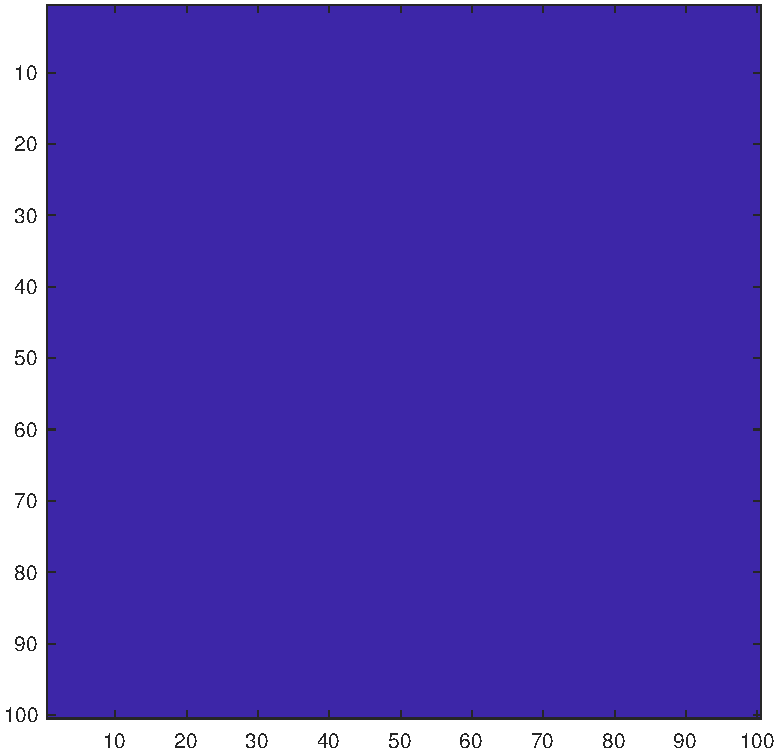
\includegraphics[height=40mm]{CIC_Sig_1_Z70.pdf} \\
        (b) Large Sphere & 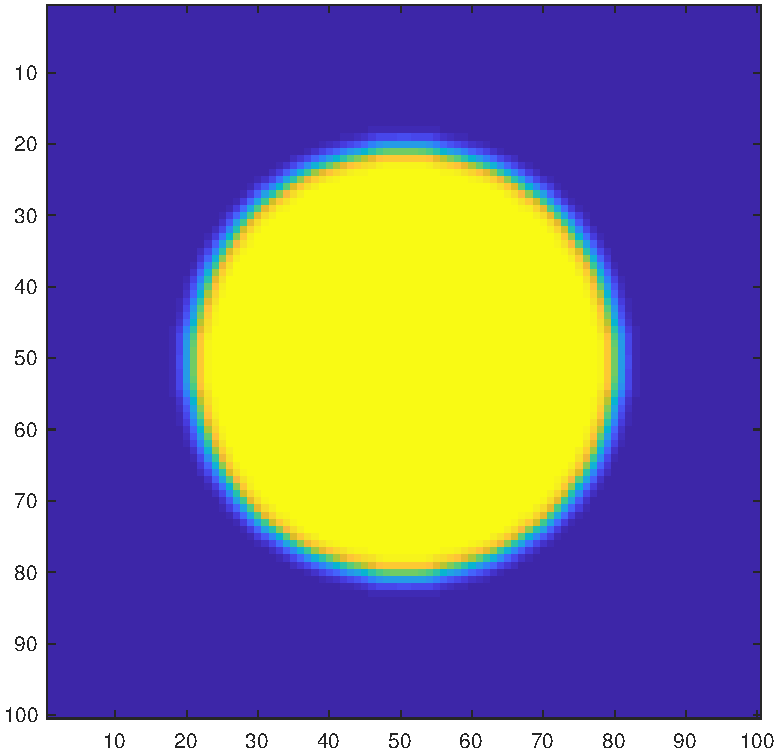
\includegraphics[height=40mm]{CIC_Sig_2_Z50.pdf} & 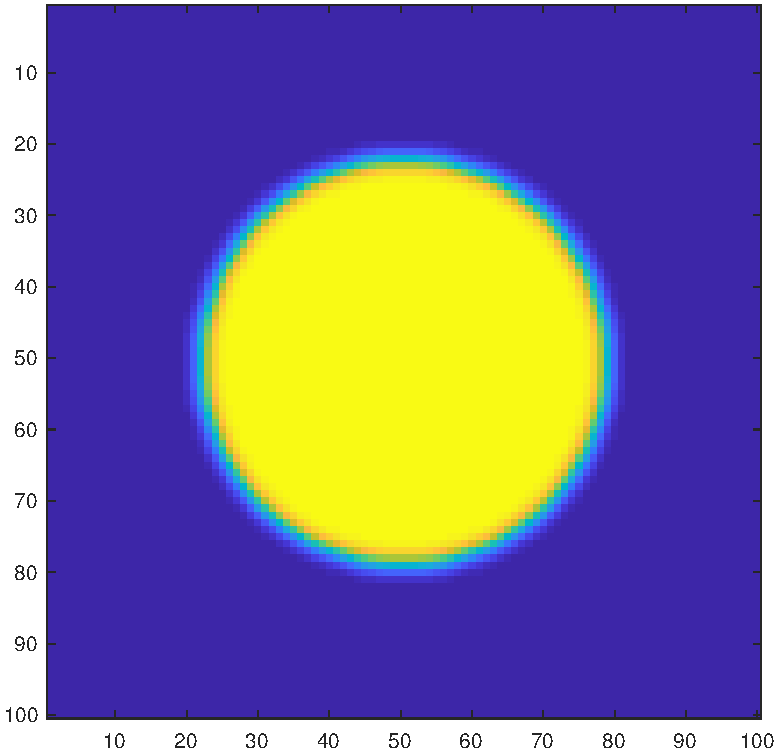
\includegraphics[height=40mm]{CIC_Sig_2_Z60.pdf} & 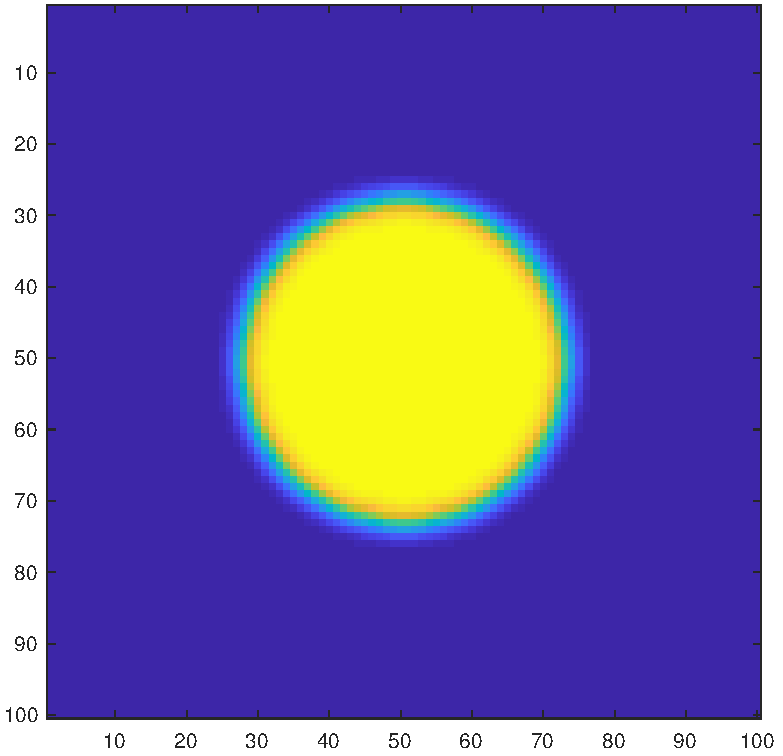
\includegraphics[height=40mm]{CIC_Sig_2_Z70.pdf} \\
        (c) Multiple Spheres & 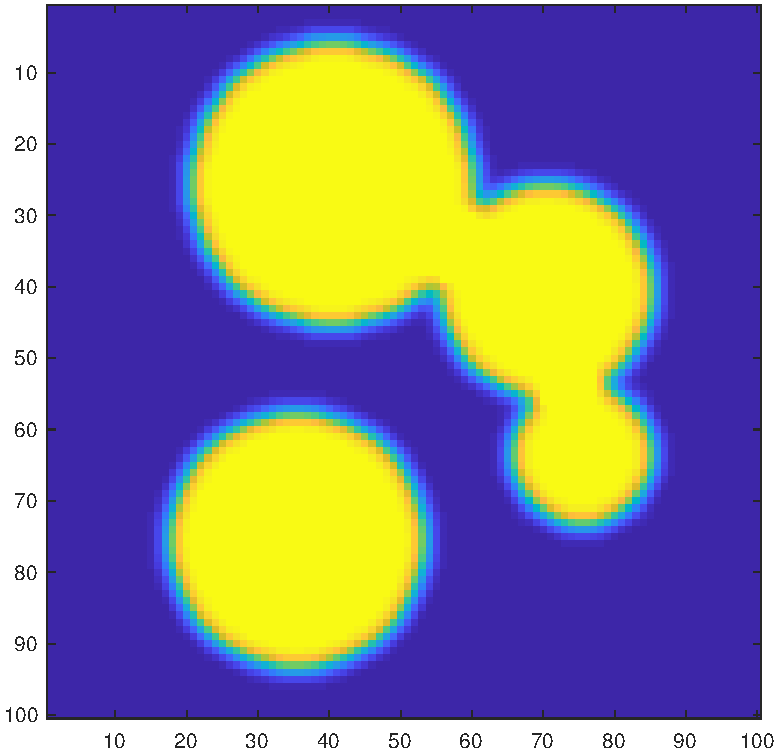
\includegraphics[height=40mm]{CIC_Sig_3_Z50.pdf} & 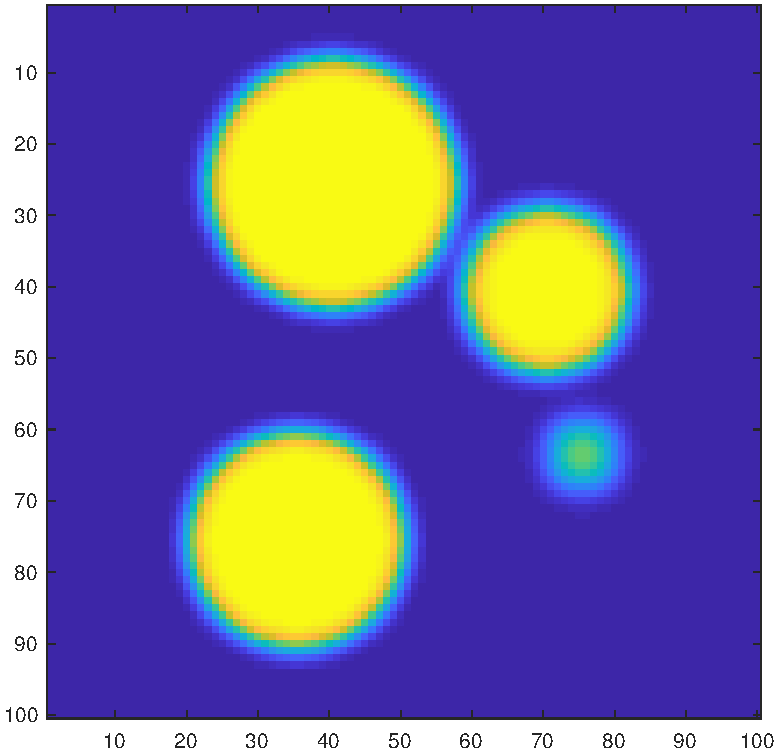
\includegraphics[height=40mm]{CIC_Sig_3_Z60.pdf} & 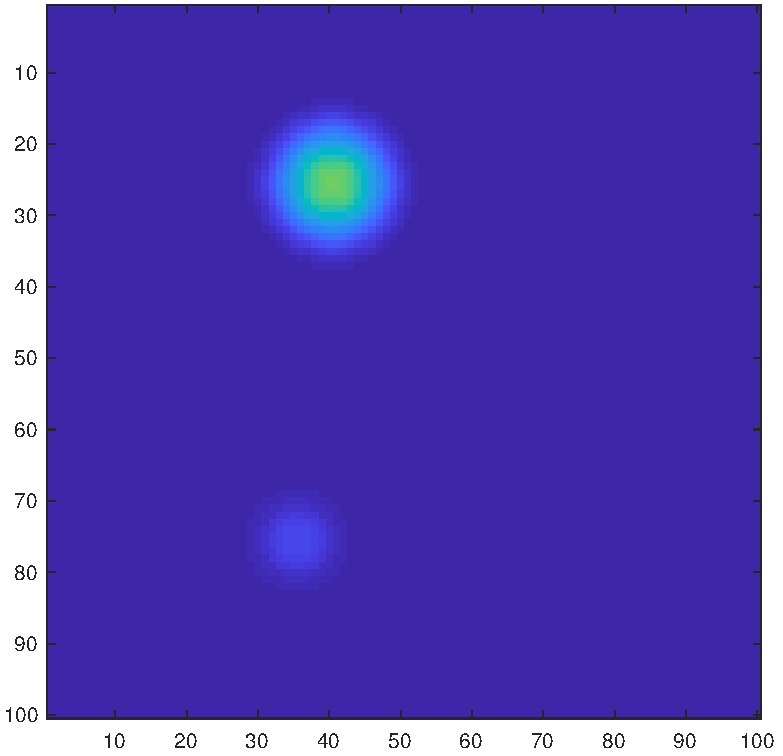
\includegraphics[height=40mm]{CIC_Sig_3_Z70.pdf} \\
        (d) UK Biobank & 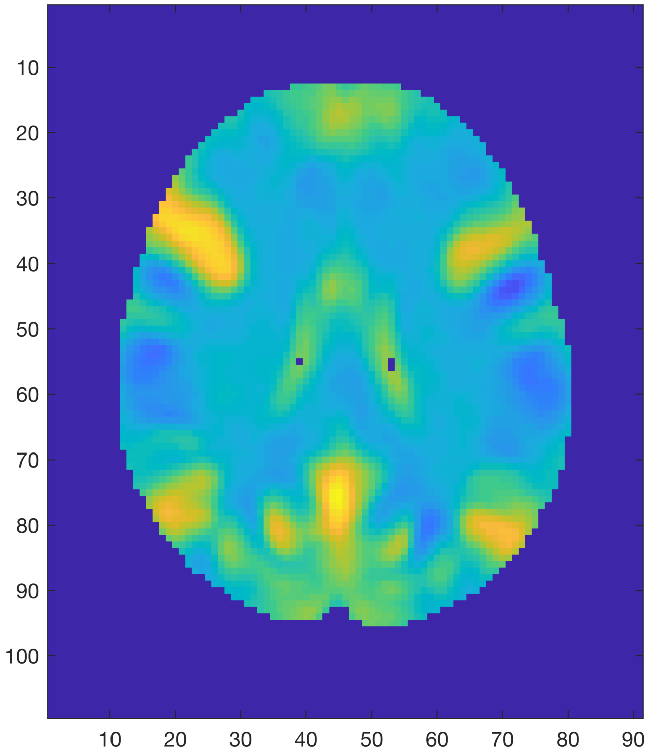
\includegraphics[height=47.5mm]{CIC_Sig_4_Z50.pdf} & 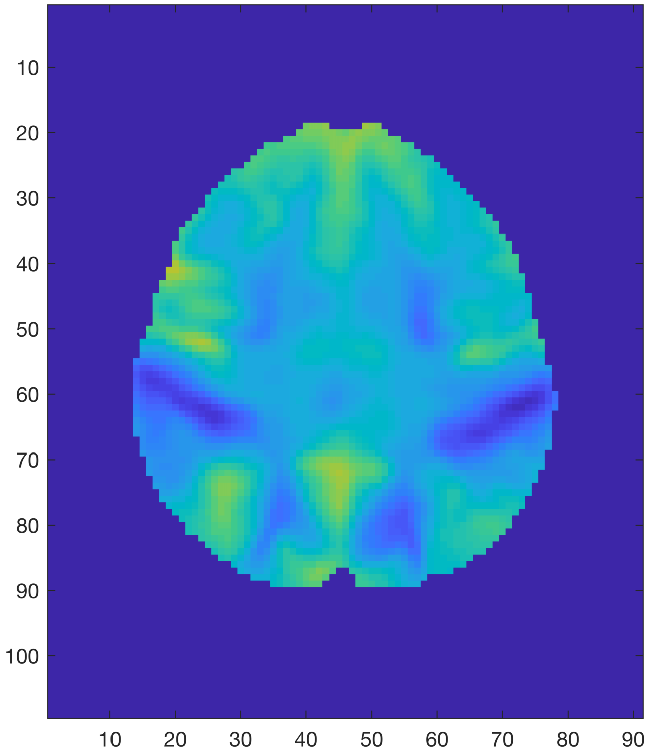
\includegraphics[height=47.5mm]{CIC_Sig_4_Z60.pdf} & 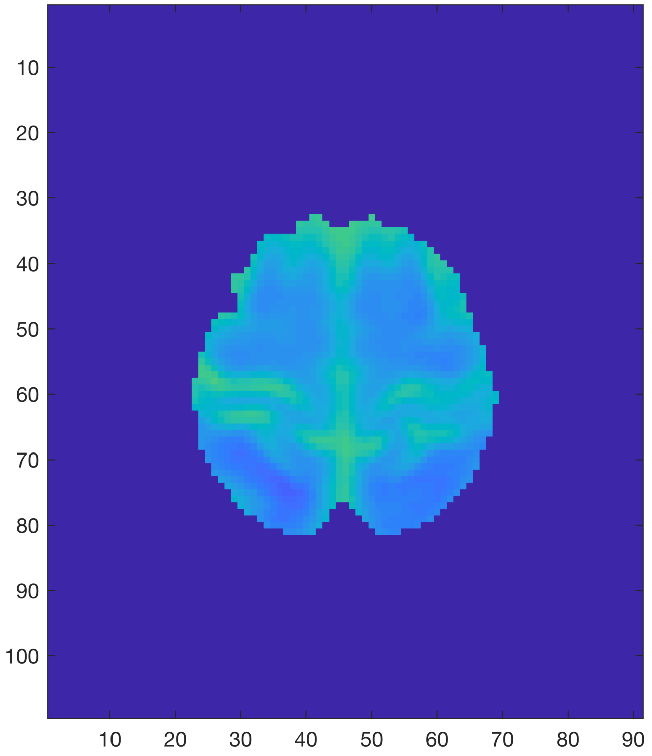
\includegraphics[height=47.5mm]{CIC_Sig_4_Z70.pdf} \\
        \bottomrule
    \end{tabular}
\end{adjustbox}
    \captionof{figure}{Four of the Cohen's $d$ fields $d(\bm{s})$ used for the 3D simulations. In (a) to (c), we show the Cohen's $d$ field for the three different spherical effects $\mu(\bm{s})$ when Gaussian noise with spatially homogeneous standard deviation was added to the signal. In (d) we show the Cohen's $d$ field corresponding to the UK Biobank full mean and standard deviation images. Note that the colormap limits for the first three Cohen's $d$ effect-size images are from 0 to 1, while the colormap limits for the UK Biobank image is from -0.8 to 0.8.}
    \label{tbl:Cohens_d_3D_figures}
\end{table}

Once again, we smoothed the noise field using a 3 voxel FWHM Gaussian kernel; since the Biobank maps were written with voxel sizes of 2mm$^{3}$, this is analogous to applying 6mm FWHM smoothing to the noise field of the original data. 

In Figure \ref{tbl:Cohens_d_3D_figures}, we show the true underlying Cohen's $d$ fields for the three synthetic 3D effects with homogeneous noise structure, and the Cohen's $d$ field corresponding to the UK Biobank full mean and standard deviation. For all four signal types, we obtained Cohen's $d$ Confidence Sets for the threshold $c = 0.8$. 

\subsection{Application to UK Biobank Data}

\section{Results}
\label{sec:simulation_results}
\subsection{2D Simulations} 
\label{sec:2D_sim_results}

Empirical coverage results for each of the three algorithms are presented for the linear ramp signal in Fig.\ \ref{fig:Cohen_2D_sig_1_results} and for the circular signal in Fig.\ \ref{fig:Cohen_2D_sig_2_results}. In both figures, on the top row we display the coverage results obtained when the standard deviation field of the noise was homogeneous across the region (corresponding to Fig.\ \ref{fig:linear_ramp_homo} for the linear ramp, Fig.\ \ref{fig:circle_homo} for the circle), and on the bottom row we display the equivalent results when the standard deviation field was spatially heterogeneous (Fig.\ \ref{fig:linear_ramp_hetero} and Fig.\ \ref{fig:circle_hetero} for the linear ramp and circle respectively). Coverage results obtained with Algorithm \ref{alg:one}.\ are displayed with a red curve, Algorithm \ref{alg:two}.\ with a blue curve, and Algorithm \ref{alg:three}.\ with a magenta curve.

For the linear ramp, across all confidence levels $1 - \alpha = 0.80, 0.90,$ and $0.95$ we generally observed valid, over-coverage for all three algorithms, particularly when larger sample sizes were used. In all plots, it appears that the coverage rates for the three algorithms are converging to the same value, slightly above the nominal target. Specifically, for the nominal target level of 80\%, in both the homogeneous and heterogeneous cases all empirical results seem to be converging to around 88\% (Fig.\ \ref{fig:Cohen_2D_sig_1_results}, left-side plots). For the 95\% target, the scale of disagreement between the empirical results and the nominal target is smaller; here, all coverage results hover close to 96\% for $N = 240$ and $480$ (Fig.\ \ref{fig:Cohen_2D_sig_1_results}, right-side plots).

While for larger sample sizes the performance of all three algorithms was similar, there was greater disparity between the methods for simulations using the small sample size of $N = 60$. Here, the empirical coverage results for Algorithm \ref{alg:one}.\ were consistently higher than the other two methods, and at the same time, results for Algorithm \ref{alg:two}.\ were always the smallest. Notably, unlike the other two methods, the empirical coverage rate for Algorithm \ref{alg:two}.\ fell below the nominal level in all simulations with a sample size of $N = 60$. 

For the circular signal, on-the-whole all three methods performed very well. In this instance, almost all empirical results for Algorithm \ref{alg:two}.\ and Algorithm \ref{alg:three}.\ lied within the 95\% confidence interval of the nominal coverage rate (blue and magenta curves sandwiched between black dashed lines for all plots in Fig.\ \ref{fig:Cohen_2D_sig_2_results}), with Algorithm \ref{alg:two}.\ performing marginally better. While we observed slight over-coverage with the three methods for $N = 60$, most substantially in simulations using the 80\% nominal target (Fig.\ \ref{fig:Cohen_2D_sig_2_results}, left-side plots), empirical coverage converged towards the nominal level for all three algorithms.

Finally, the use of homogeneous or heterogeneous noise in the model had minimal impact on any of the algorithm's empirical coverage performance for either of the signals. This is exemplified in Figs.\ \ref{fig:Cohen_2D_sig_1_results} and \ref{fig:Cohen_2D_sig_2_results}, where in both cases the homogeneous coverage plots presented in the top row are almost identical to the corresponding heterogeneous plots shown below. 

\begin{figure}[!htbp]
\hspace*{-3.0cm}
\centering
    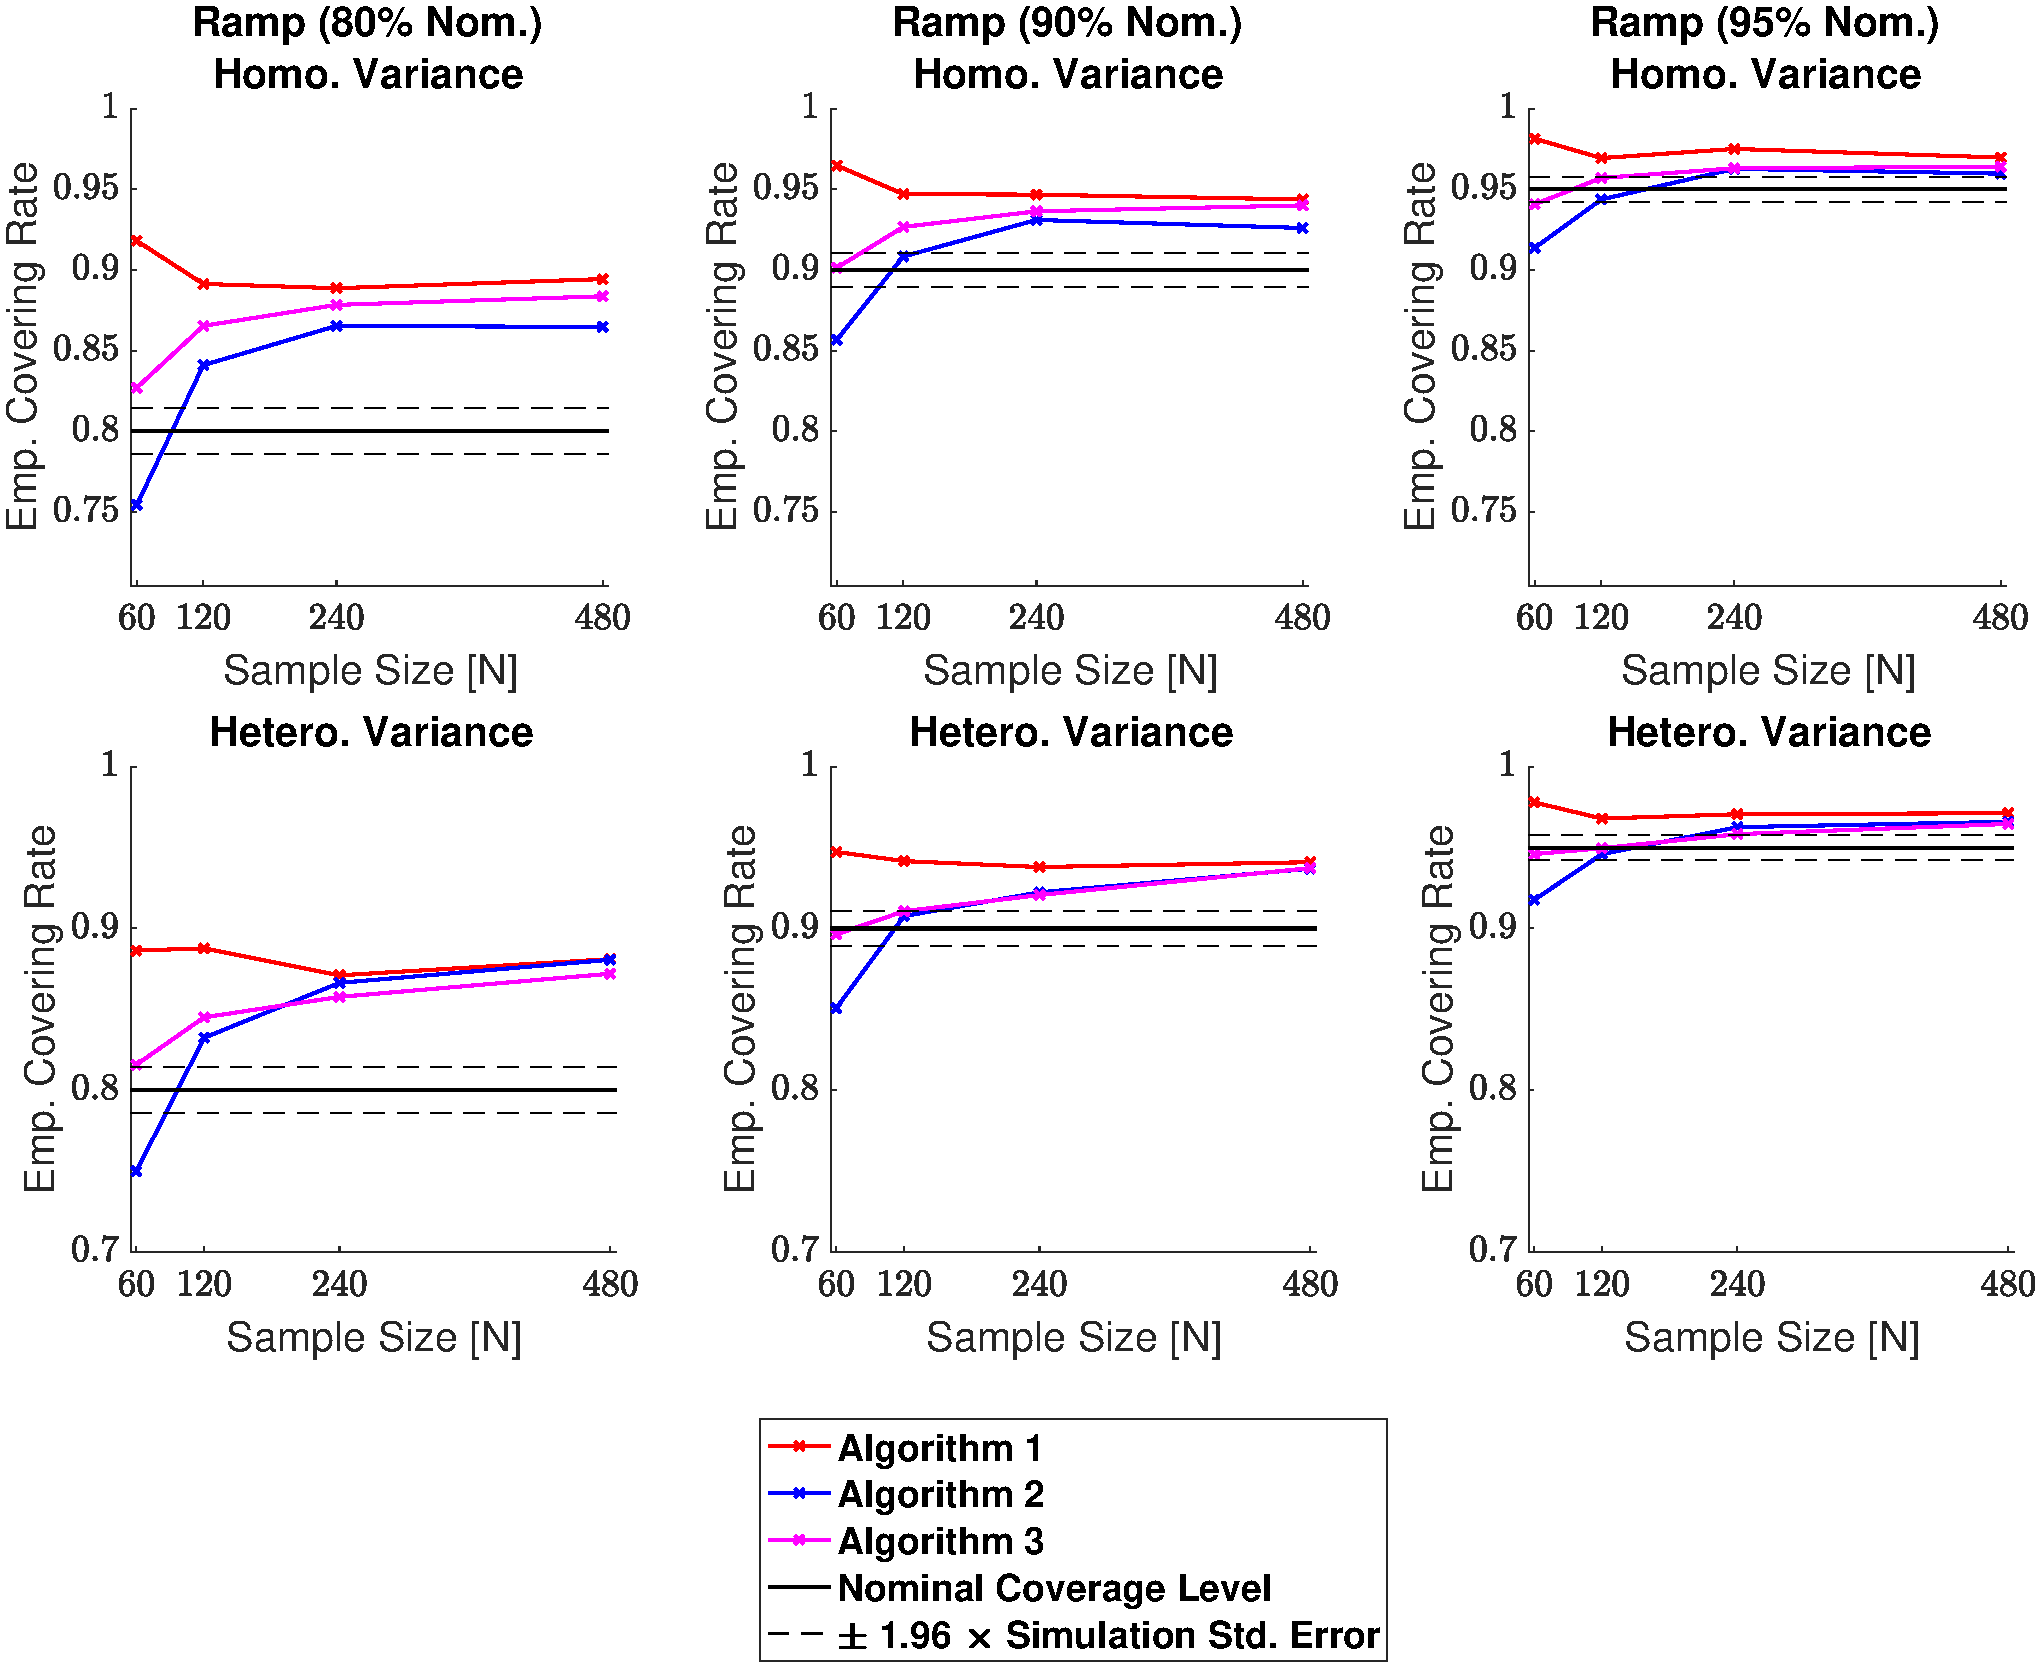
\includegraphics[height=6.1in]{CIC_2D_sig_1_results.pdf}
\caption{Coverage results for the linear ramp signal, with homogeneous (top row) and heterogeneous (bottom row) Gaussian noise structures. For large sample sizes the empirical coverage performance of all three algorithms was similar, hovering slightly above the nominal level in all simulations. For $N = 60$ the degree of over-coverage became larger for Algorithm \ref{alg:one}., while empirical coverage for Algorithm \ref{alg:two}.\ fell below the nominal target. Algorithm \ref{alg:three}.\ performed best, with all results remaining particularly close to the nominal target level for simulations using a 95\% confidence level (right plots).}
\label{fig:Cohen_2D_sig_1_results}
\end{figure}

\begin{figure}[!htbp]
\hspace*{-3.0cm}
\centering
    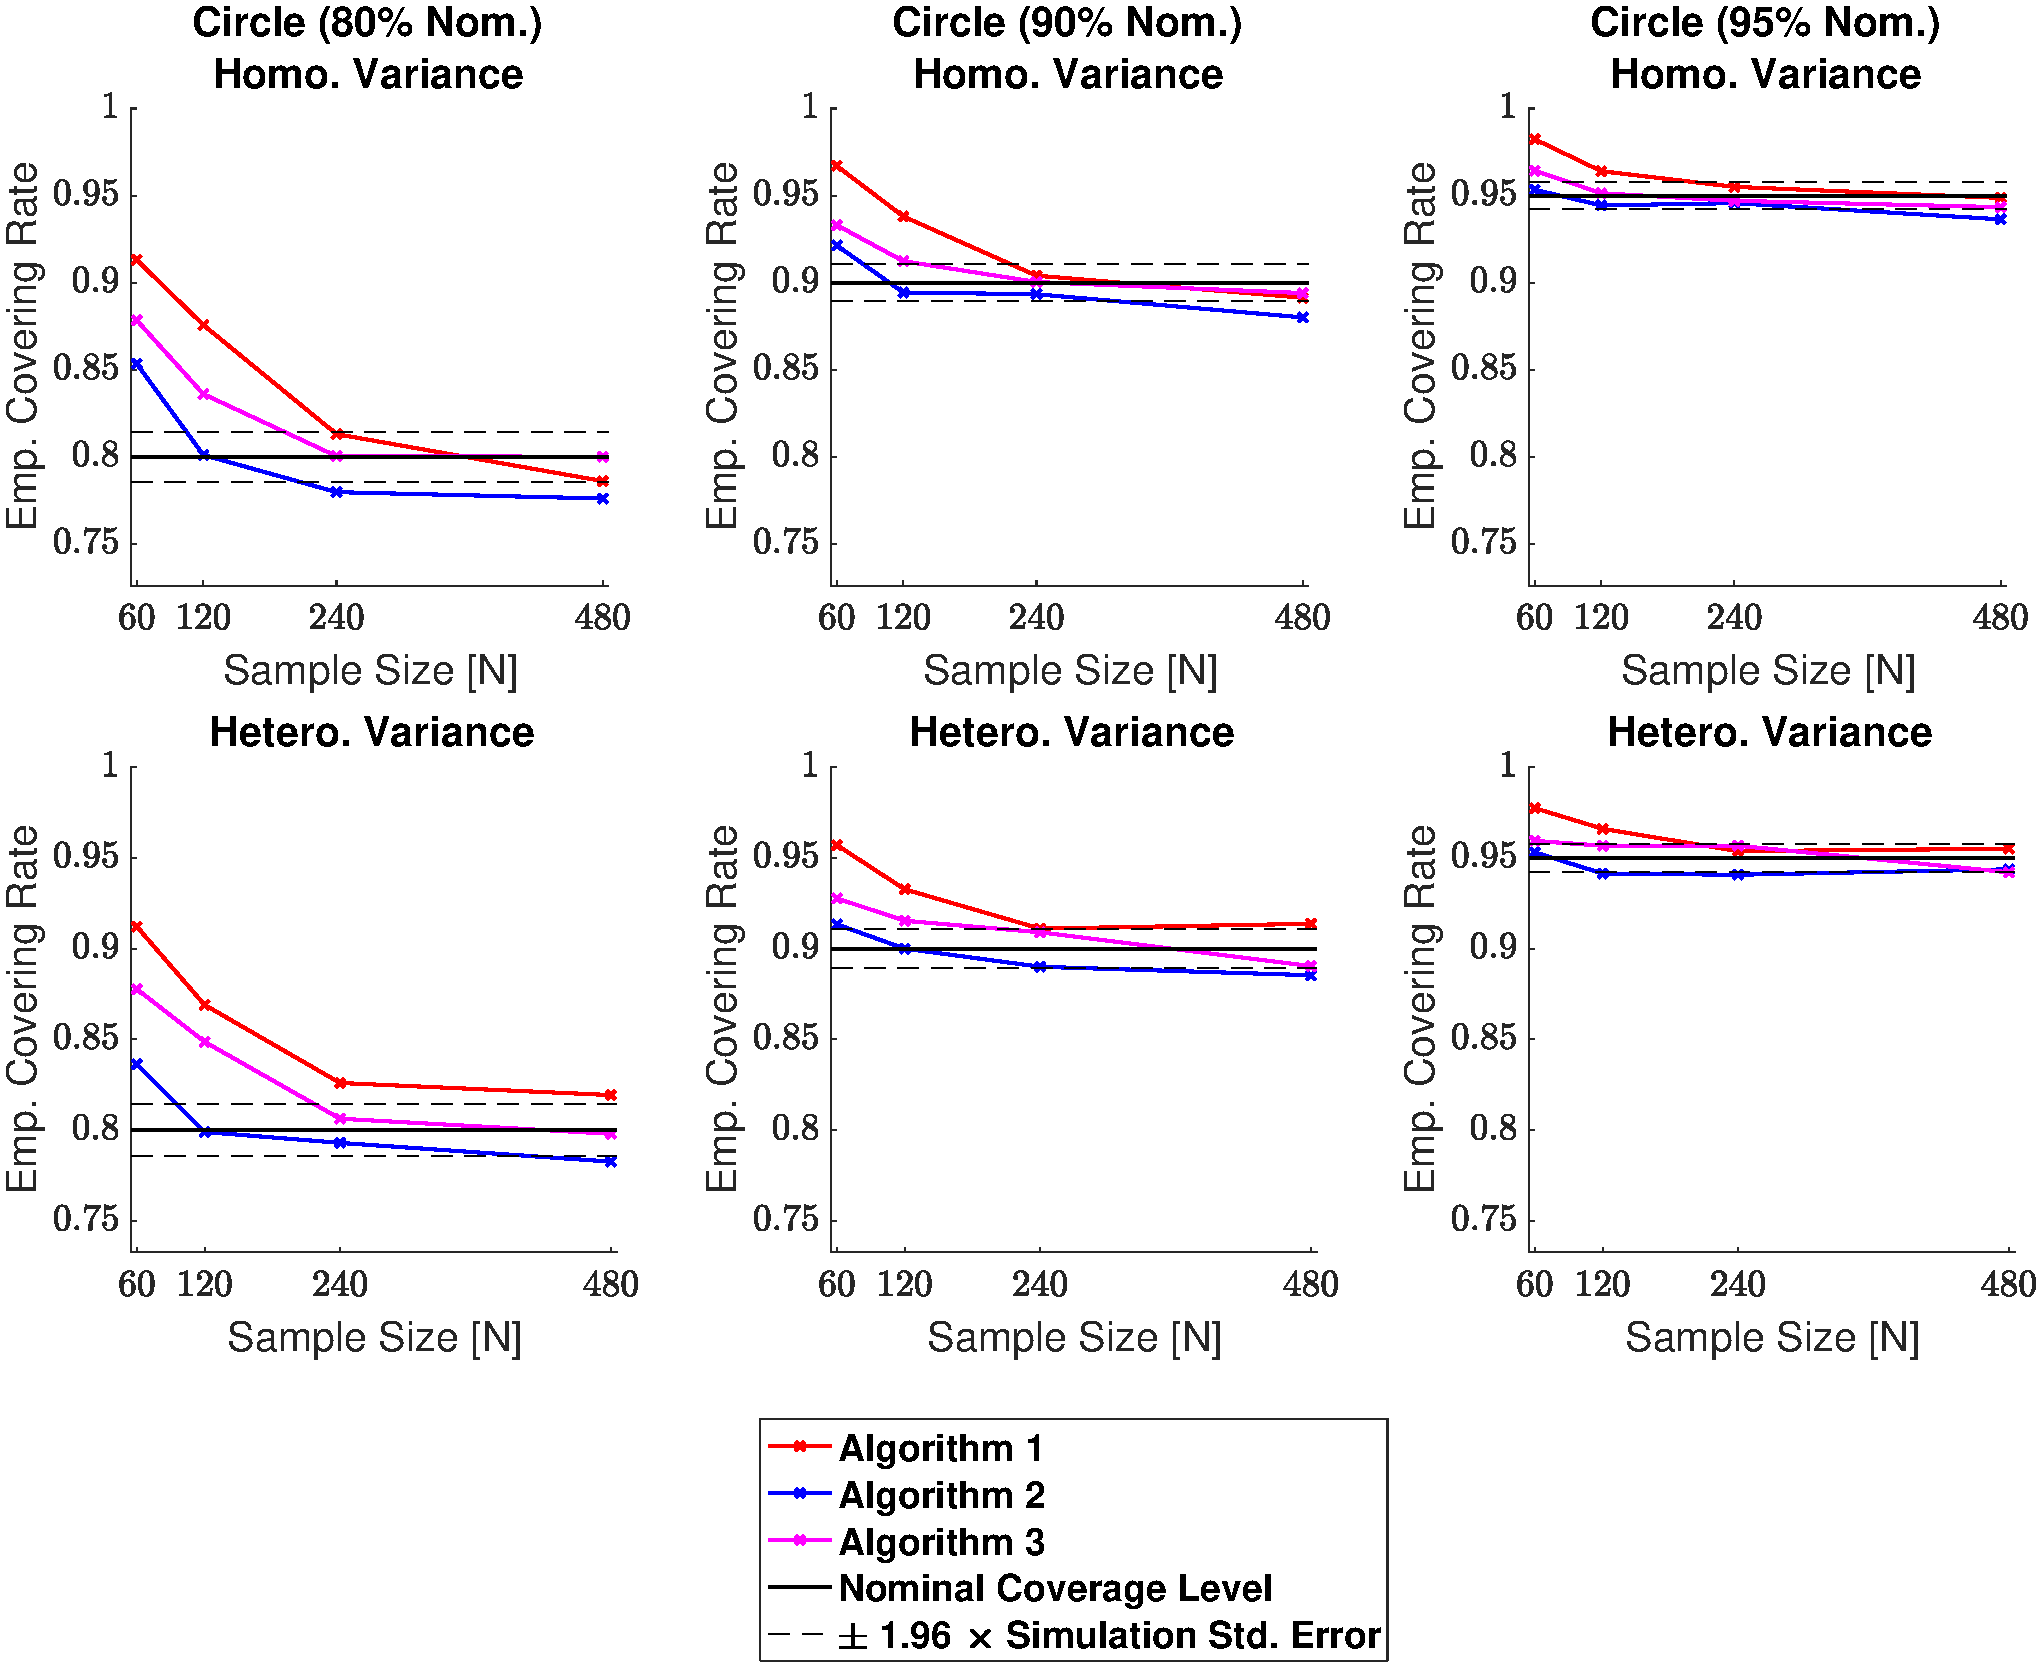
\includegraphics[height=6.1in]{CIC_2D_sig_2_results.pdf}
\caption{Coverage results for the circular signal, with homogeneous (top row) and heterogeneous (bottom row) Gaussian noise structures. All algorithms performed very well, and unlike the linear ramp, empirical coverage for all three methods converged towards the nominal level. For smaller sample sizes there was a slight degree of over-coverage, most noticeably for simulations using the 80\% nominal target. Overall, Algorithm \ref{alg:two}.\ performed marginally better than the other two methods, and Algorithm \ref{alg:one}.\ performed the worst.}
\label{fig:Cohen_2D_sig_2_results}
\end{figure}

\clearpage

\subsection{3D Simulations} 
\label{sec:3d_sim_results}
Empirical coverage results for each of the three algorithms are presented in Figs.\ \ref{fig:Cohen_3D_sig_1_results}, \ref{fig:Cohen_3D_sig_2_results}, \ref{fig:Cohen_3D_sig_3_results} and \ref{fig:Cohen_3D_sig_4_results} respectively for each of the four 3D signal types displayed in Fig.\ \ref{tbl:Cohens_d_3D_figures} (small sphere, large sphere, multiple spheres, UK Biobank). For the spherical effects (Figs. \ref{fig:Cohen_3D_sig_1_results}, \ref{fig:Cohen_3D_sig_2_results} and \ref{fig:Cohen_3D_sig_3_results}), on the top row we display the coverage results obtained when the standard deviation field of the noise was homogeneous across the region, and on the bottom row we display the equivalent results when the standard deviation field was spatially heterogeneous. For the UK Biobank signal (Fig.\ \ref{fig:Cohen_3D_sig_4_results}), the full standard deviation image computed from the UK Biobank data was used for the standard deviation field of the noise, and hence in this case there is only one row of results. Once again, coverage results obtained with Algorithm \ref{alg:one}.\ are displayed with a red curve, Algorithm \ref{alg:two}.\ with a blue curve, and Algorithm \ref{alg:three}.\ with a magenta curve.

Across all 3D simulations, we observed consistencies between the results obtained with each of the three algorithms: In general, empirical coverage for all methods came above the nominal target, and similar to the 2D simulations, the extent of over-coverage was smaller when a larger confidence level was used. Comparing the three methods, coverage results for Algorithm \ref{alg:one}.\ were considerably higher than the other two methods, particularly when a small sample size and confidence level were used. For the `large sphere' and `multiple spheres' signal types, Algorithm \ref{alg:one}.\ suffered with over-coverage of above 15\% in simulations with a sample of size of $N = 60$ and a nominal target level of 80\% (Figs.\ \ref{fig:Cohen_3D_sig_2_results} and \ref{fig:Cohen_3D_sig_3_results}, left-side plots). For both of these signals, there was still a considerable amount of over-coverage when larger sample sizes of $N = 240$ and $480$ were used. On the other hand, Algorithm \ref{alg:two}.\ and Algorithm \ref{alg:three}.\ performed similarly in large sample sizes across all simulations, with empirical coverage results coming slightly above the nominal target. Notably, both of these algorithms performed very well for simulations with a 95\% nominal target level (all figures, right-side plots).
Differences between these two methods were more distinguished for smaller sample sizes of $N = 60$ and $120$, where coverage results for Algorithm \ref{alg:two}.\ were moderately less than Algorithm \ref{alg:three}. Consequentially, Algorithm \ref{alg:two}.'s results came closer to the nominal target here, although for the `multiple sphere' and `UK Biobank' signal types, in some cases Algorithm \ref{alg:two}.'s results fell \textit{below} the nominal level (Figs. \ref{fig:Cohen_3D_sig_3_results} and \ref{fig:Cohen_3D_sig_4_results}). Overall, empirical coverage for Algorithm \ref{alg:three}.\ was the most uniform of the three methods with respect to changes in sample size. 

Comparing Figs.\ \ref{fig:Cohen_3D_sig_1_results} and \ref{fig:Cohen_3D_sig_2_results}, we observed a slight deterioration in the performance of all three algorithms when moving from the small sphere signal type to the large sphere. In particular, results obtained from applying the three methods to the large sphere fell further above the nominal target relative to the small sphere. This was most severe for Algorithm \ref{alg:one}., where differences between the two sets of results were larger than 10\% for the 80\% confidence level (Figs.\ \ref{fig:Cohen_3D_sig_1_results} and \ref{fig:Cohen_3D_sig_2_results}, left-side plots). These differences were comparatively marginal for Algorithm \ref{alg:two}.\ and Algorithm \ref{alg:three}., where we observed only a slight increase in empirical coverage. This would suggest that both of these methods are fairly robust to changes in the boundary length.

Finally, the use of homogeneous or heterogeneous noise in the model once again had very little impact on the performance of all three algorithms. Nonetheless, for simulations with small sample sizes, a heterogeneous noise structure lead to a slight decrease in the empirical coverage results for Algorithm \ref{alg:two}.\ and Algorithm \ref{alg:three}.\ (Figs. \ref{fig:Cohen_3D_sig_1_results}, \ref{fig:Cohen_3D_sig_2_results} and \ref{fig:Cohen_3D_sig_3_results}, left-side plots).

\begin{figure}[!htbp]
\hspace*{-3.0cm}
\centering
    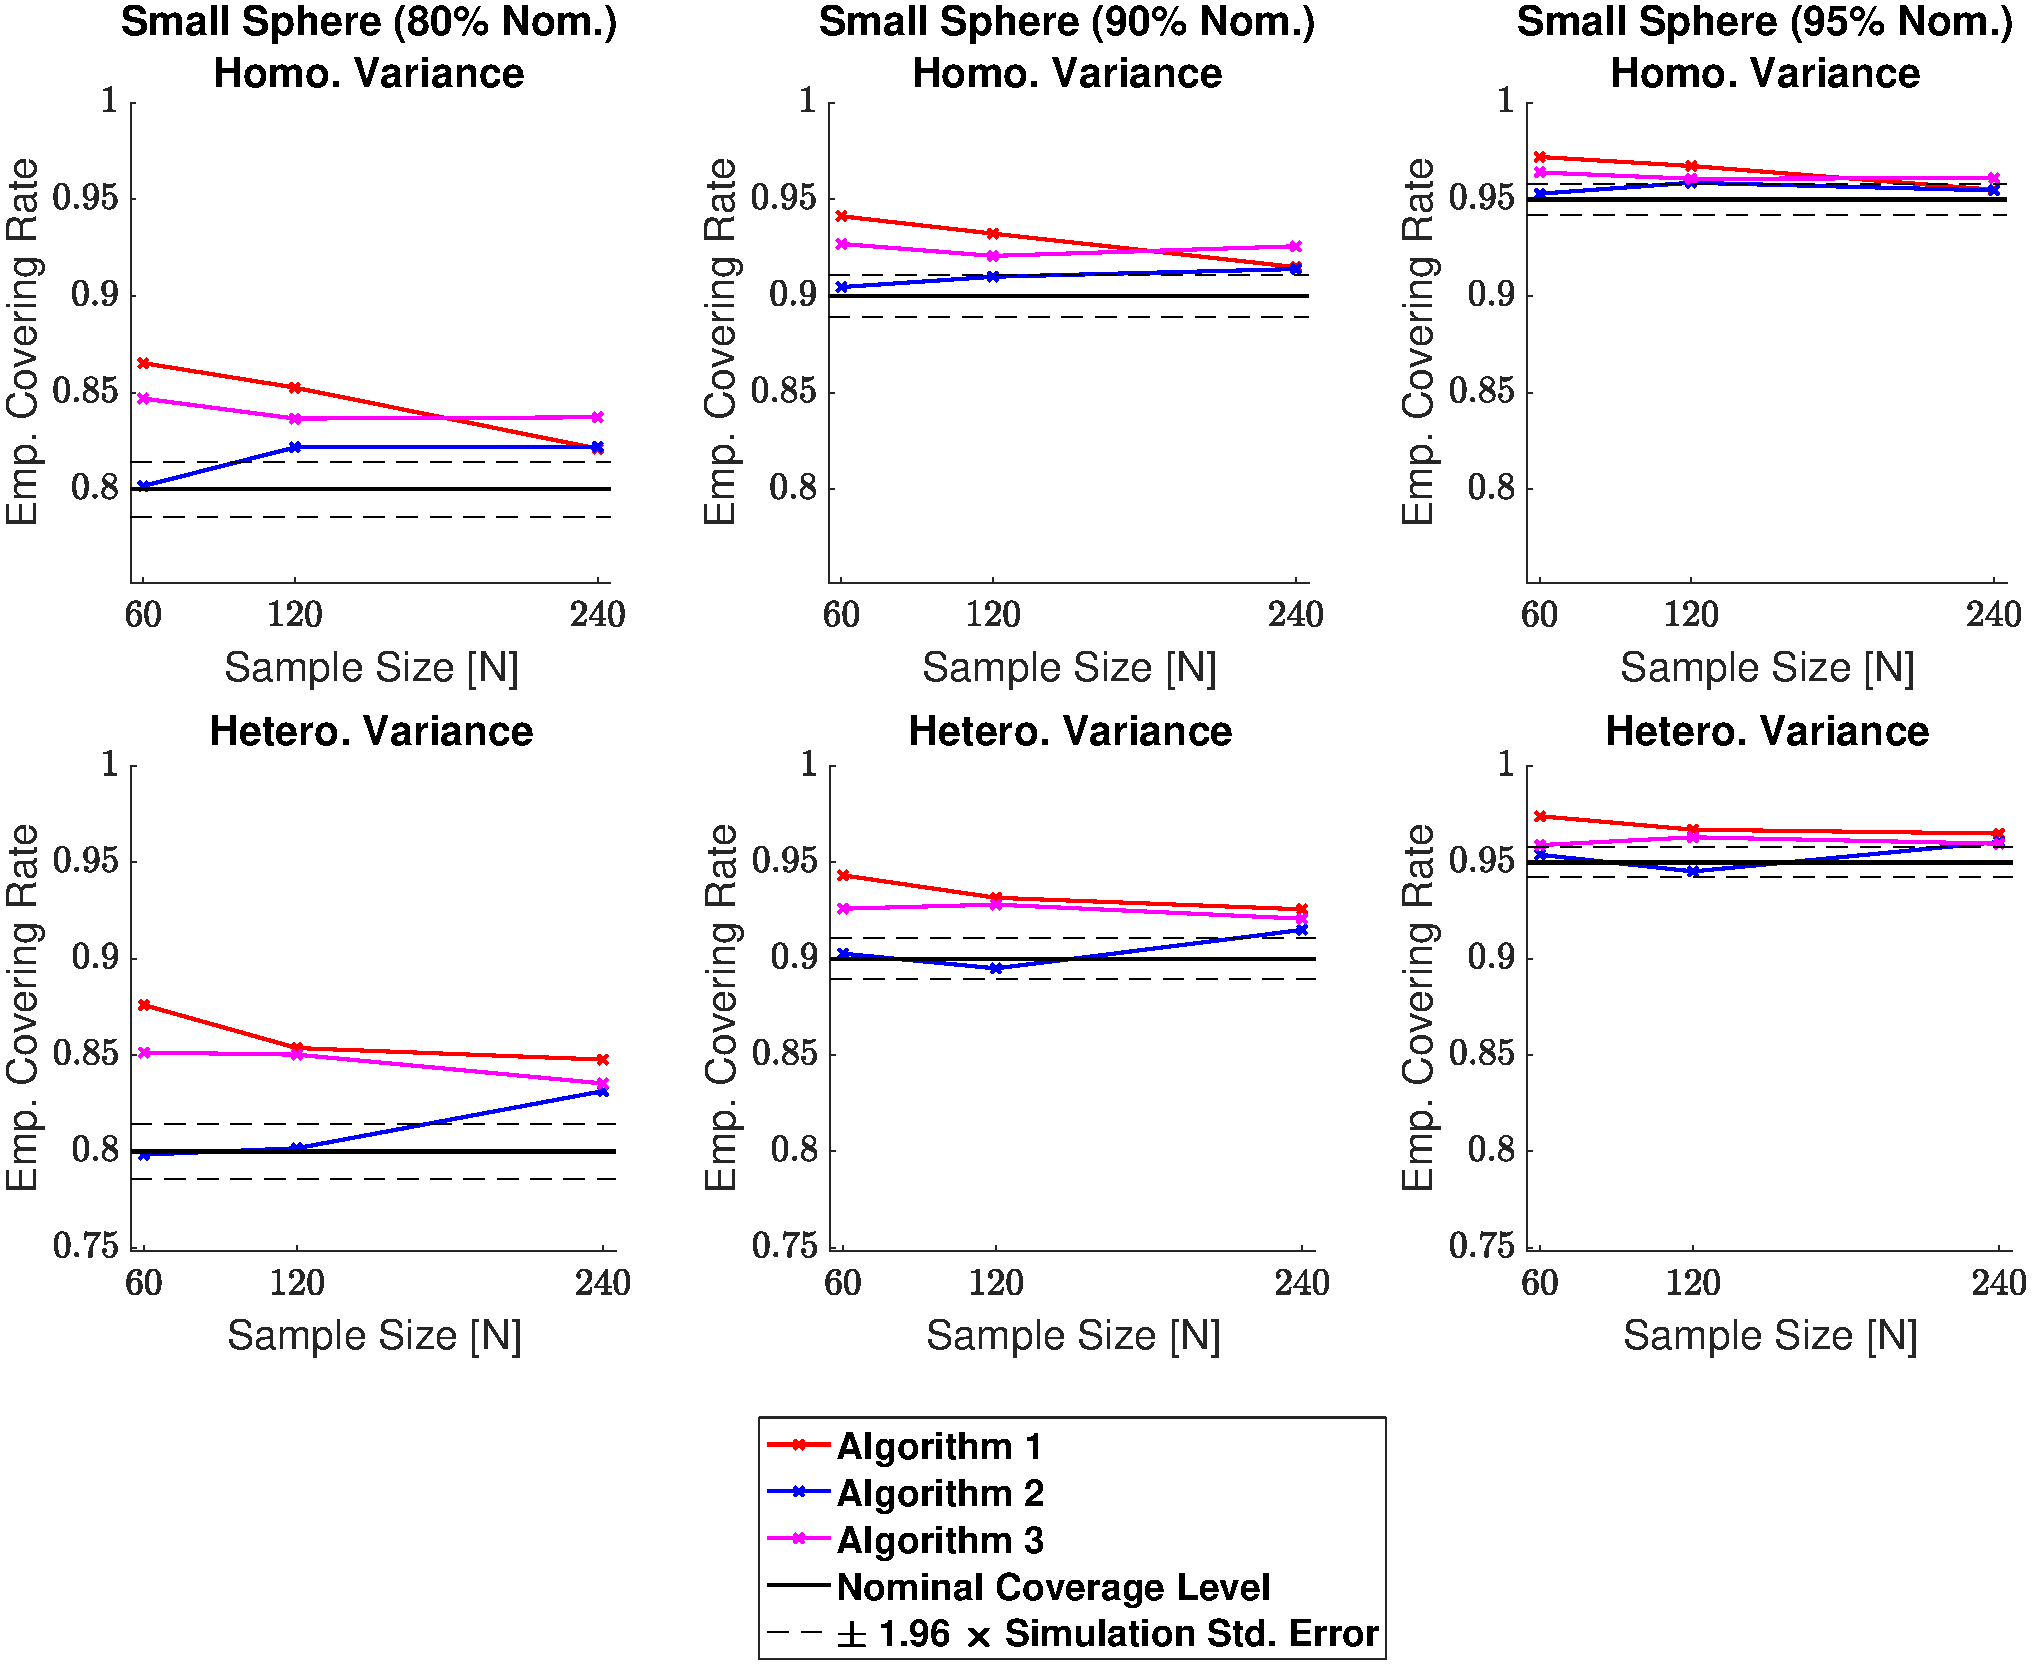
\includegraphics[height=6.1in]{CIC_3D_sig_1_results.pdf}
\caption{Coverage results for the small sphere signal type, with homogeneous (top row) and heterogeneous (bottom row) Gaussian noise structures. In general, empirical coverage remained above the nominal level across all simulations, and for the 95\% confidence level (right plots), the results of all three methods fell close to the nominal target. All methods were robust as to whether the subject-level noise had homogeneous or heterogeneous variance structure. Because of this, there are minimal differences comparing the plots between both rows.}
\label{fig:Cohen_3D_sig_1_results}
\end{figure}

\begin{figure}[!htbp]
\hspace*{-3.0cm}
\centering
    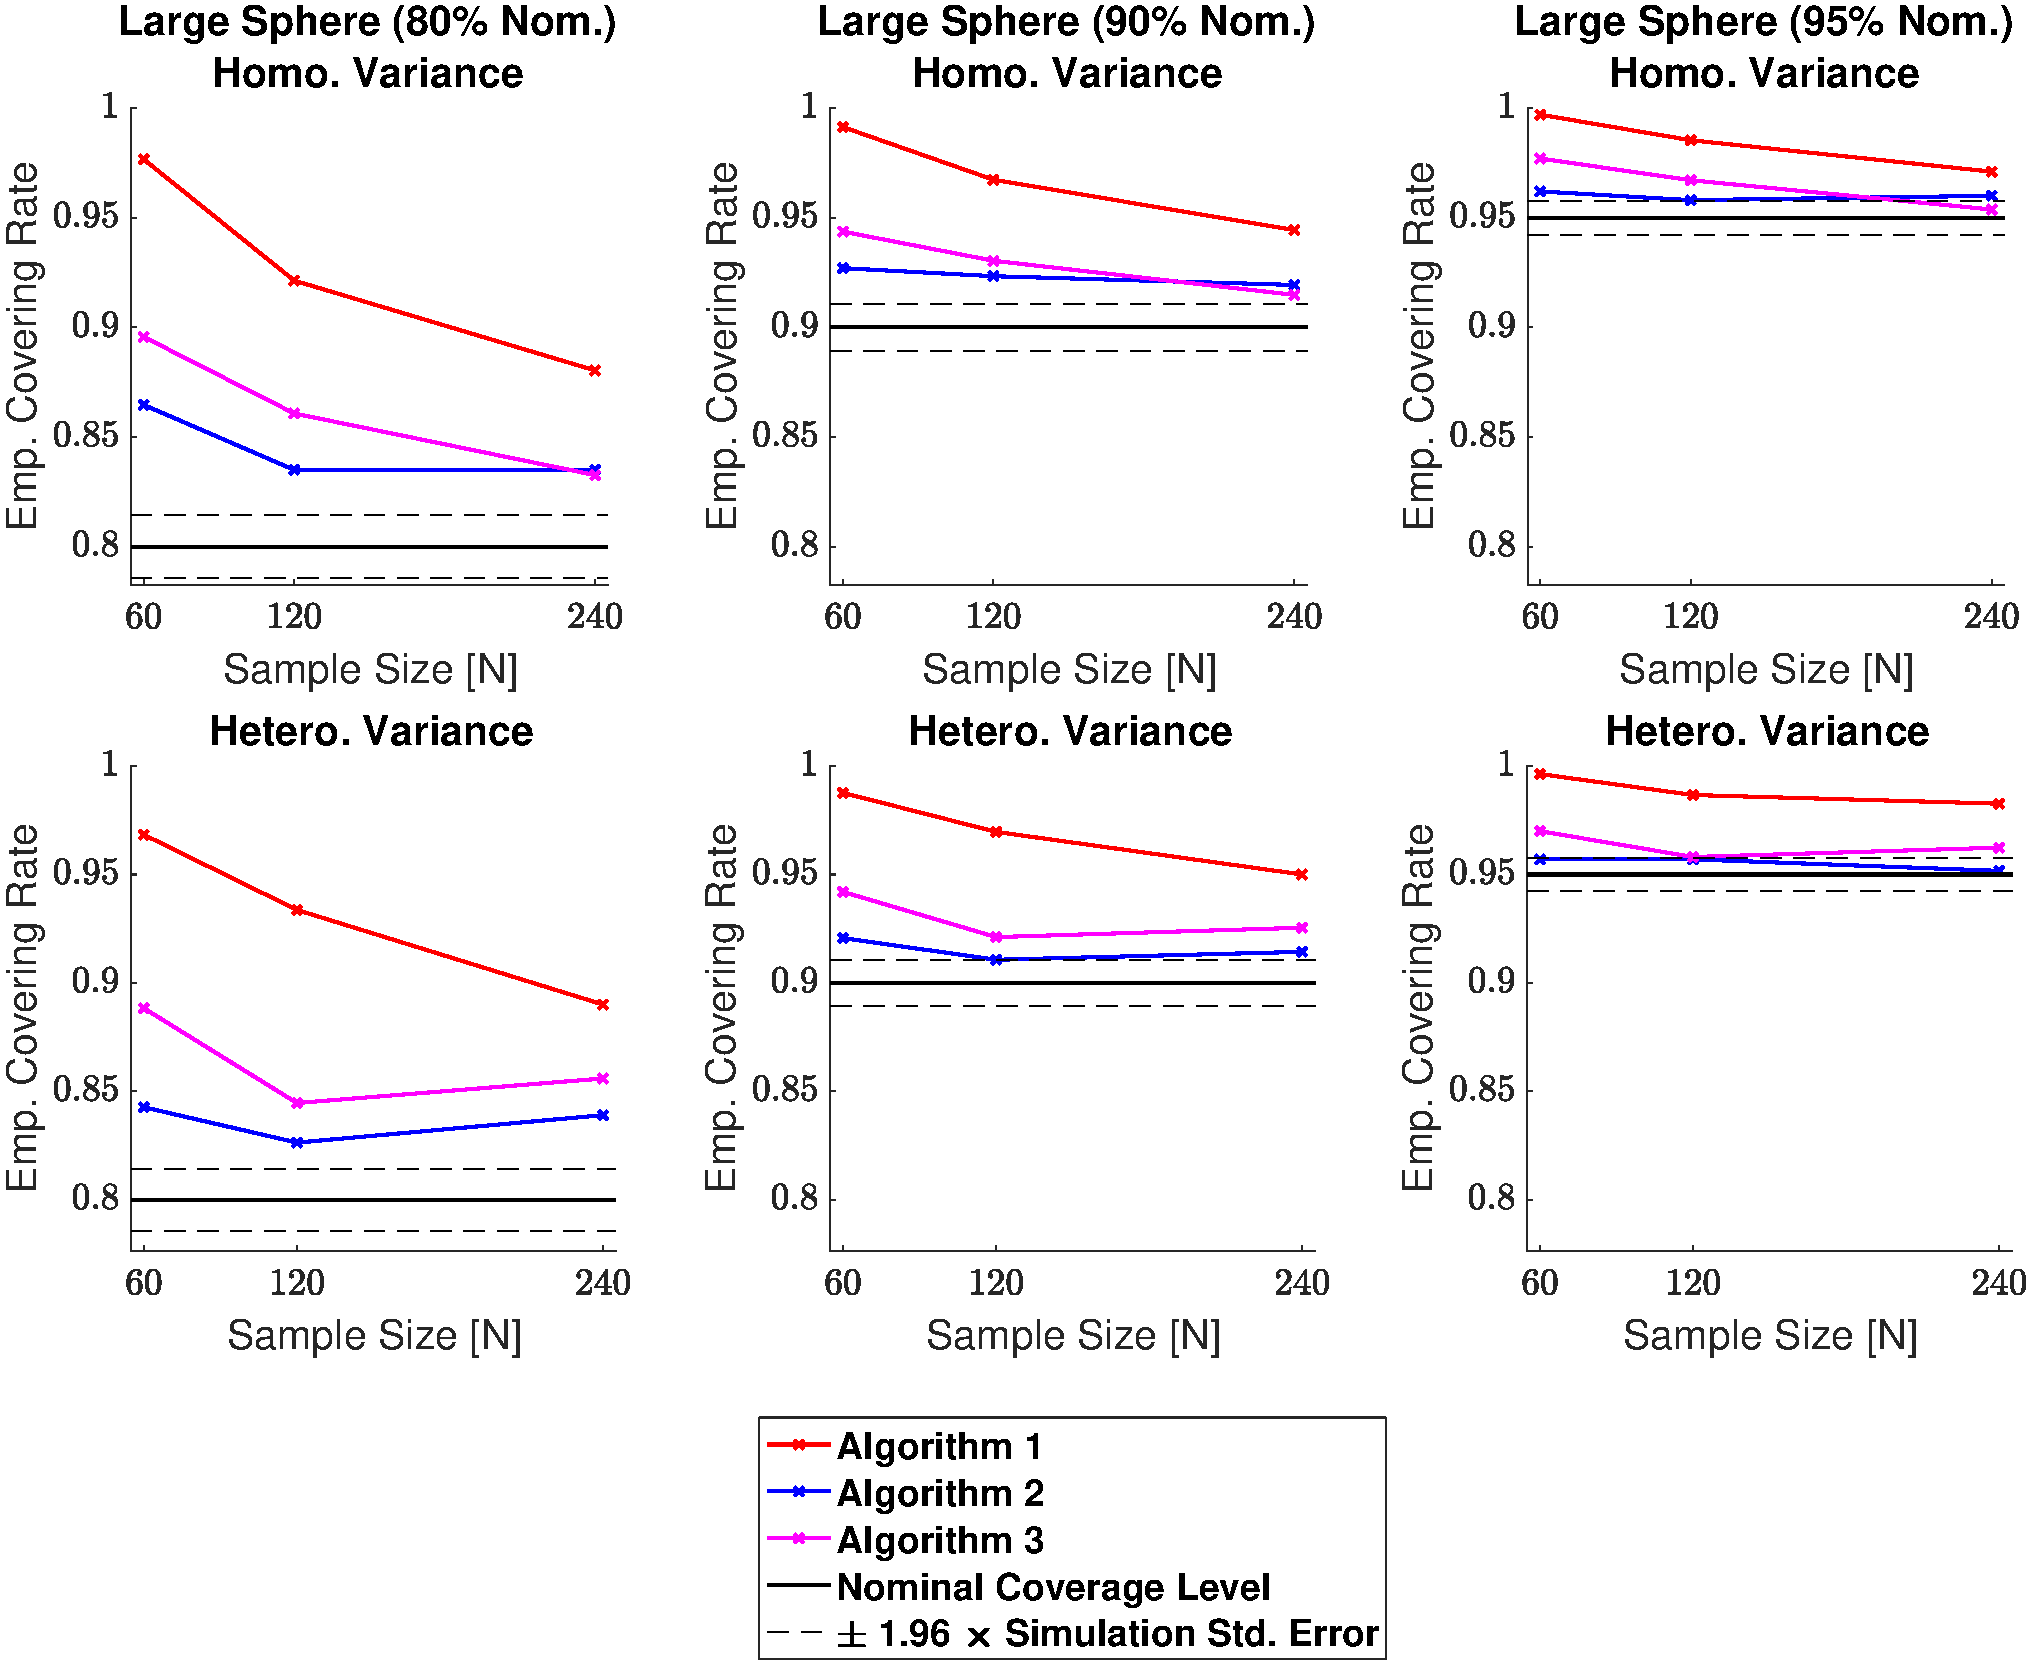
\includegraphics[height=6.1in]{CIC_3D_sig_2_results.pdf}
\caption{Coverage results for the large sphere signal type, with homogeneous (top row) and heterogeneous (bottom row) Gaussian noise structures. Compared with the small sphere results displayed in Fig.\ \ref{fig:Cohen_3D_sig_2_results}, empirical coverage results were higher for all three methods here. Algorithm \ref{alg:one}.\ suffered from a particularly large degree of over-coverage for simulations with a small sample size. Coverage performance for Algorithm \ref{alg:two}.\ and Algorithm \ref{alg:three}.\ was closer in resemblance to the corresponding small sphere results, with Algorithm \ref{alg:two}.\ performing slightly better. This suggests that both of these methods are fairly robust to changes in the boundary length.} 
\label{fig:Cohen_3D_sig_2_results}
\end{figure}

\begin{figure}[!htbp]
\hspace*{-3.0cm}
\centering
    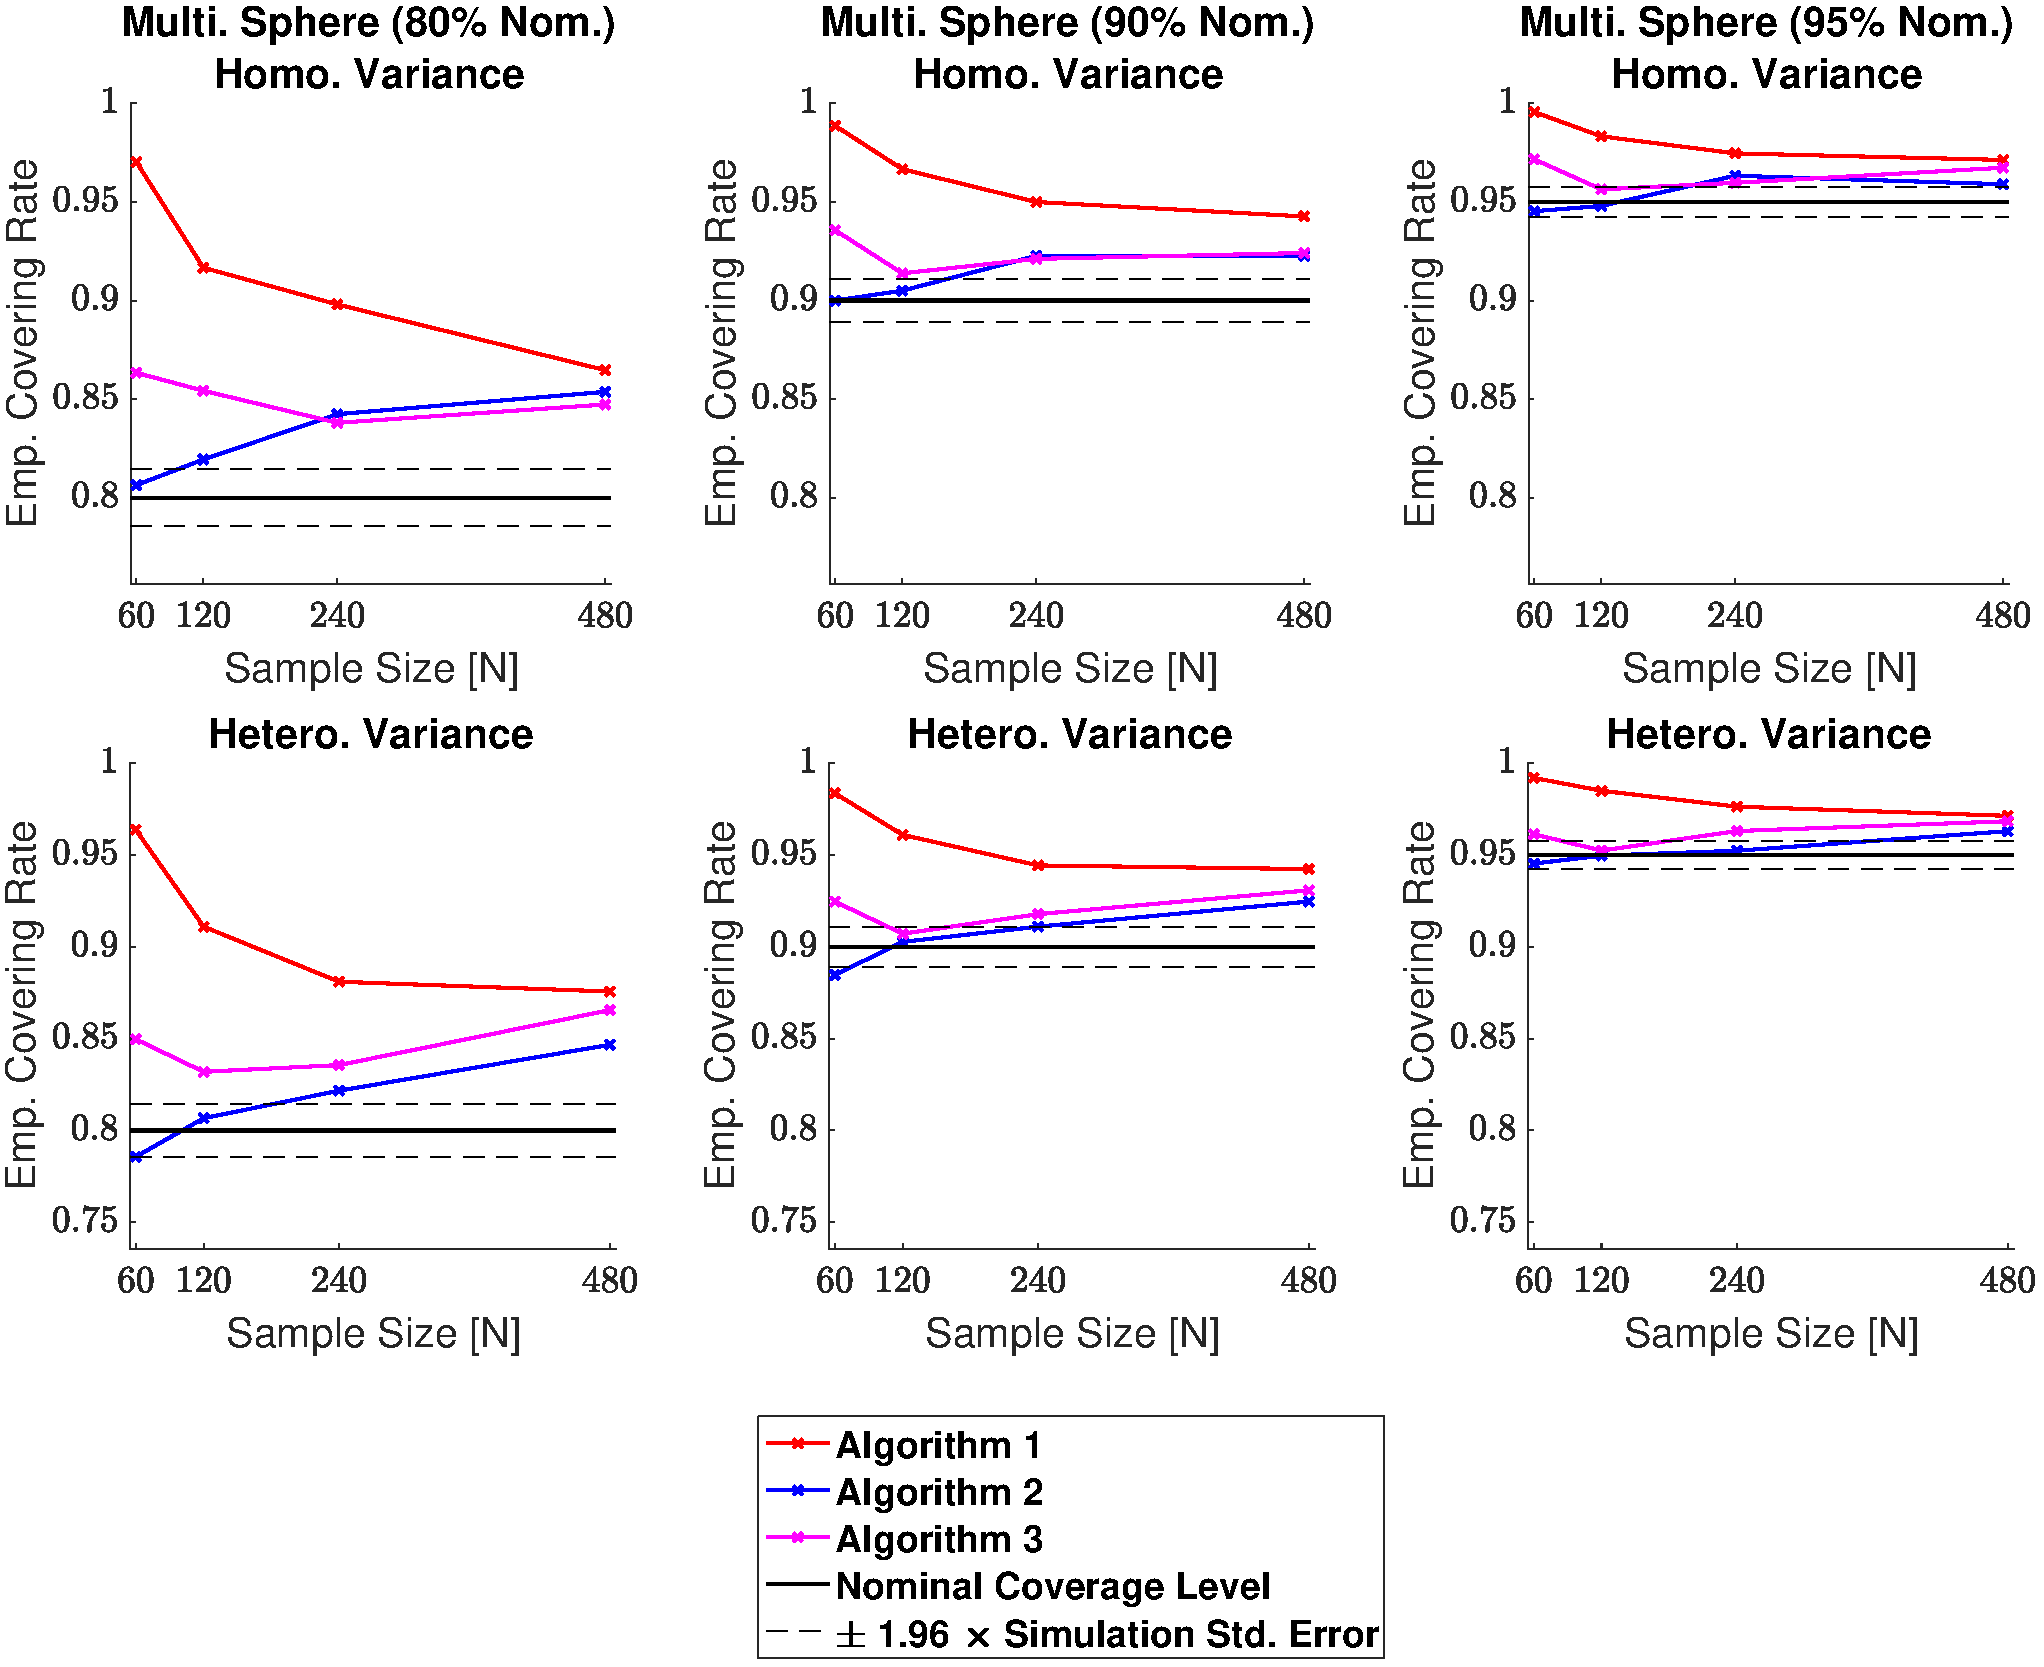
\includegraphics[height=6.1in]{CIC_3D_sig_3_results.pdf}
\caption{Coverage results for the multiple spheres signal type, with homogeneous (top row) and heterogeneous (bottom row) Gaussian noise structures. Algorithm \ref{alg:two}.\ and Algorithm \ref{alg:three}.\ both performed well, particularly for the 95\% confidence level, where coverage levels remained in the vicinity of the 95\% confidence interval of the nominal target. While Algorithm \ref{alg:two}.\ was closer to the nominal target for $N = 60$, in some cases empirical coverage went slightly below the nominal level. In comparison to the other two methods, Algorithm \ref{alg:one}.\ suffered from a large degree of over-coverage, which slightly improved as the sample size increased.}
\label{fig:Cohen_3D_sig_3_results}
\end{figure}

\begin{figure}[!htbp]
\hspace*{-3.0cm}
\centering
    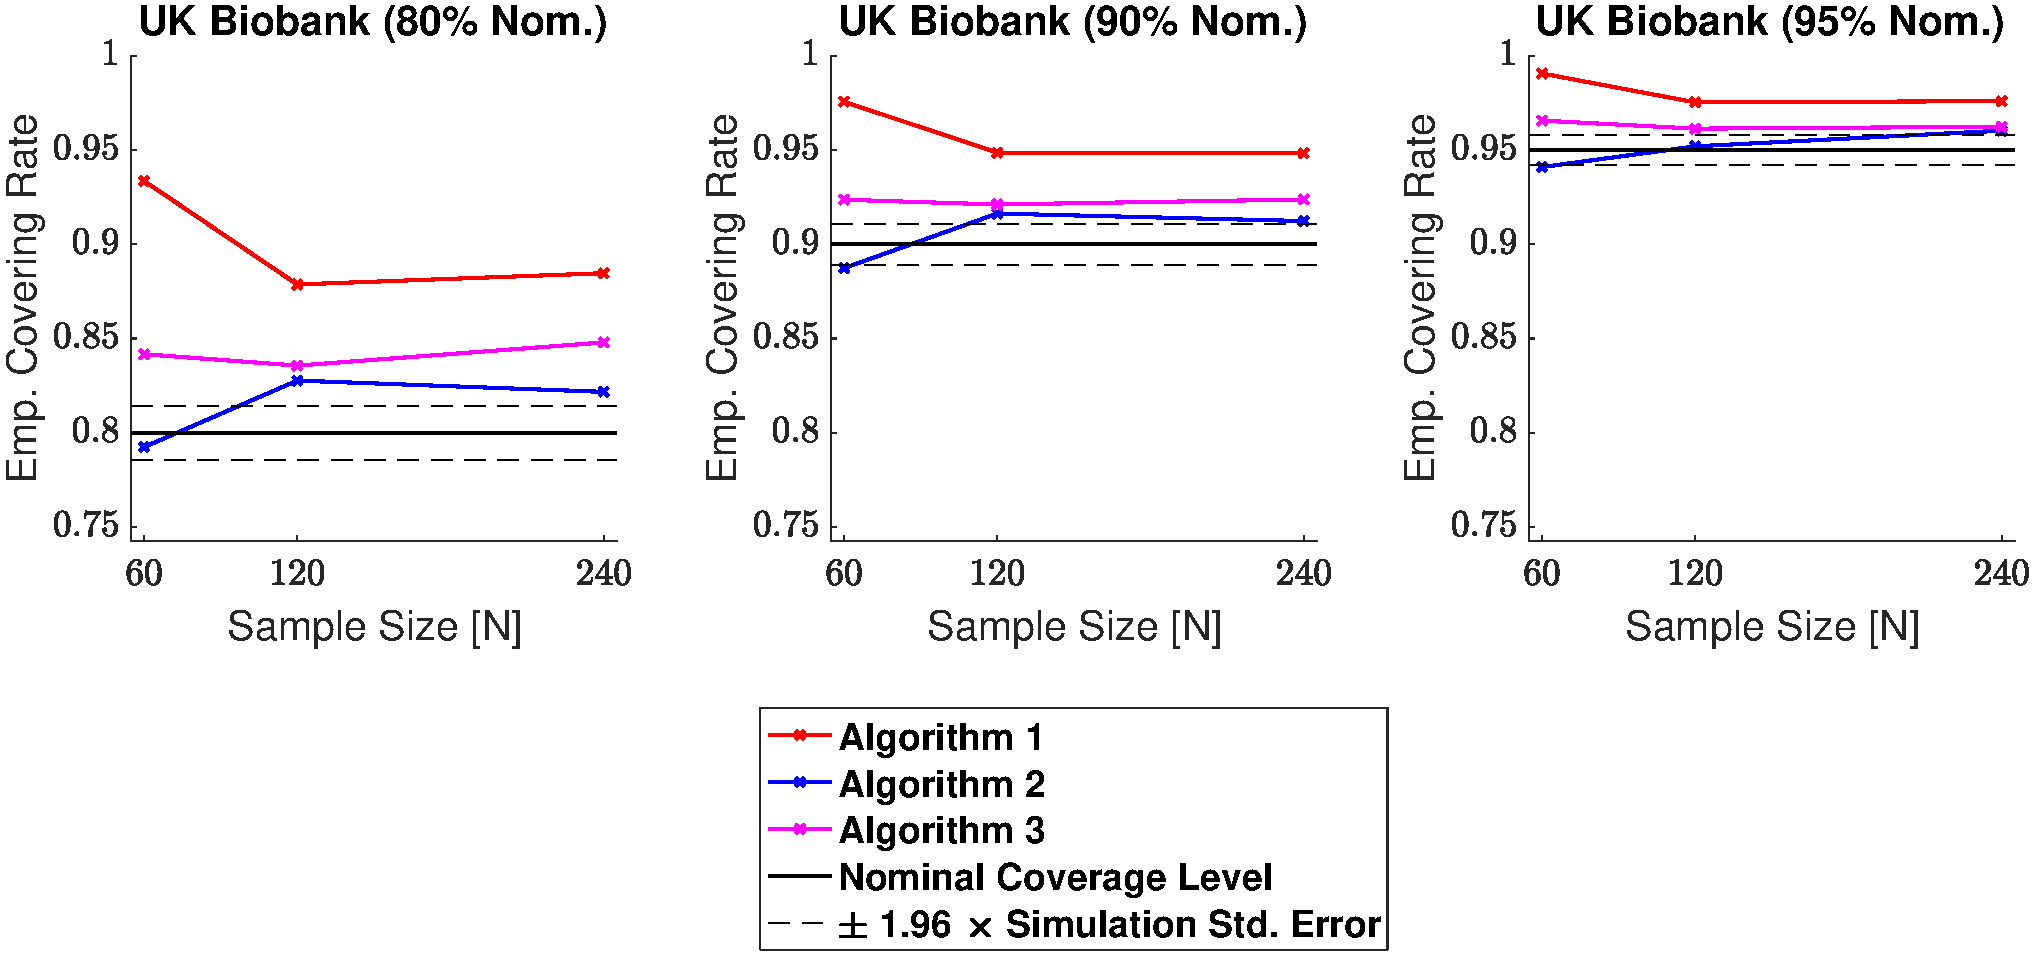
\includegraphics[width=7.4in]{CIC_3D_sig_4_results.pdf}
\caption{Coverage results for the UK Biobank signal type, where the full standard deviation image was used as the standard deviation of the subject-level noise fields. Covereage results here were similar to the results for the multiple spheres signal type shown in Fig.\ \ref{fig:Cohen_3D_sig_3_results}. Once again, both Algorithm \ref{alg:two}.\ and Algorithm \ref{alg:three}.\ performed well, with empirical coverage rates hovering above the nominal target for large sample sizes, while results for Algorithm \ref{alg:one}.\ came further above the nominal level.}
\label{fig:Cohen_3D_sig_4_results}
\end{figure}

\clearpage

\subsection{Human Connectome Project} 
Cohen's $d$ Confidence Sets obtained by applying Algorithm \ref{alg:three}.\ to 80 subjects contrast data from the Human Connectome Project are shown in Fig.\ \ref{fig:HCP_Algorithm_3}. CSs computed on the same data using Algorithm \ref{alg:one}.\ and Algorithm \ref{alg:two}.\ are displayed in Figs.\ \ref{fig:HCP_Algorithm_1} and \ref{fig:HCP_Algorithm_2} respectively. For each figure, we display the CSs obtained from applying the specified algorithm with three separate thresholds, $c= 0.5, 0.8,$ and $1.2$. These three Cohen's $d$ effect sizes were classified as medium, large, and very large in \textit{\citet*{Cohen2013-it}}.

In the top plot of Fig.\ \ref{fig:HCP_Algorithm_3}, the red upper CS localized brain regions within the frontal cortex commonly associated to working memory. This included areas of the superior frontal gyrus (left and right, all slices), middle frontal gyrus (left, coronal slice), paracingulate gyrus (left and right, axial slice) and insular cortex. Other brain areas encapsulated inside the upper CS were the angular gyrus (left and right, axial slice), cerebellum (left and right, sagittal slice) and precuneus (left and right, axial slice). For all these regions, the method identified clusters of voxels where we can assert with 95\% confidence there was a Cohen's $d$ effect size greater than 0.5.

By increasing the threshold to $c = 0.8$ (Fig.\ \ref{fig:HCP_Algorithm_3}, middle plot), there was a shrinking of both the blue lower CSs and red upper CSs. Therefore, while we can confidently declare a medium effect size in all of the brain areas identified above, the quantity of voxels within each region that we can proclaim to have a large effect size is considerably smaller. In the case of the right cerebellar hemisphere (left, sagittal slice) and insular cortex, the upper CS vanished completely, indicating that the method did not locate any voxels in these regions where we can assert a Cohen's $d$ effect size greater than 0.8.

For the largest threshold assessed, $c = 1.2$, the red upper CS was empty, and hence we can not proclaim any part of the brain to to have attained a very large effect size. Notably, this is in spite of the fact that the yellow point estimate set contains a small but appreciable number of voxels, signifying that based on the data alone, these voxels were estimated to have a Cohen's $d$ effect size greater than 1.2. Conversely, the large quantity of (grey backgroud) voxels lying outside the blue lower CS in Fig.\ \ref{fig:HCP_Algorithm_3} imply an effect size \textit{less} than 1.2 across the vast majority of the brain.

In Fig.\ \ref{fig:HCP_Algorithm_3_vs_GLM}. the red upper CSs computed with Algorithm \ref{alg:three}.\ are compared with the thresholded $t$-statistic map (green-yellow voxels) obtained from applying a one-sample $t$-test group-analysis to the 80 subjects contrast data, using a voxelwise FWE-corrected threshold of $p < 0.05$. This figure demonstrates the improved spatial specificity that can be provided with the Confidence Sets in comparison to the traditional approach. Specifically, while the thresholded statistic map contains one large cluster covering a sizeable portion of the parietal lobe across both brain hemispheres, the red upper CSs pinpoint precise areas in the precuneus and angular gyrus where a practically significant medium (or large) Cohen's $d$ effect size can be inferred (Fig.\ \ref{fig:HCP_Algorithm_3_vs_GLM}, axial slices).

\begin{table}[!htbp]
\hspace*{-0.5cm}
\begin{adjustbox}{center}
\centering
    \begin{tabular}{cm{50mm}m{50mm}m{50mm}}
       \toprule
         Threshold $c$ & \hspace{1.4cm} Sagittal (X = 63) & \ \hspace{1.0cm} Coronal (Y = 130) & \hspace{0.9cm} Axial (Z = 124)\\
        \midrule
        0.5 Cohen's $d$ & 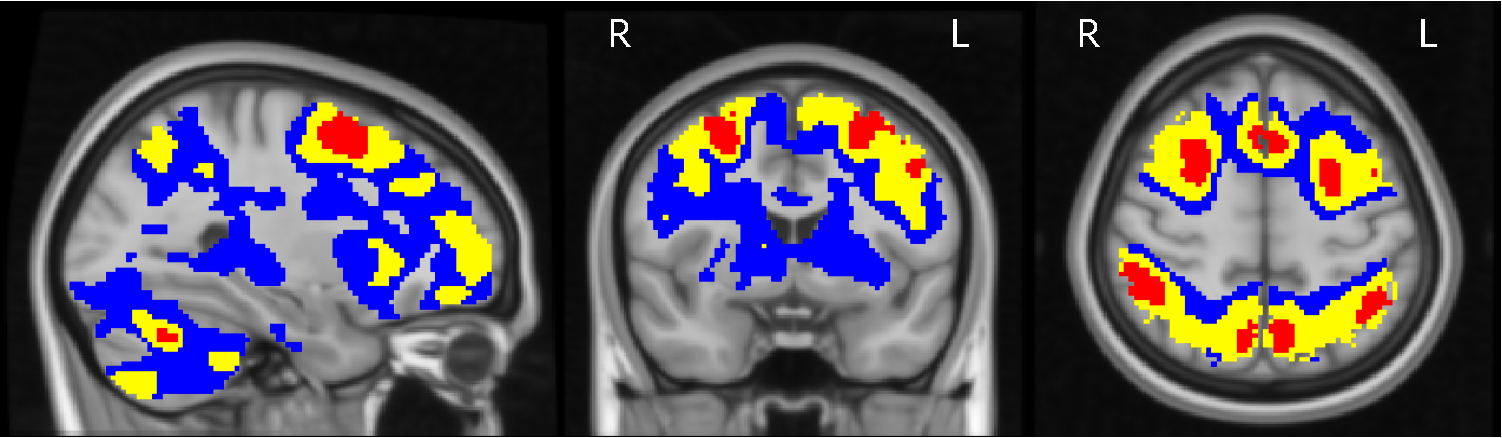
\includegraphics[height=45.5mm]{CIC_Fig1_Algorithm3_c05.pdf}\\
        0.8 Cohen's $d$ & 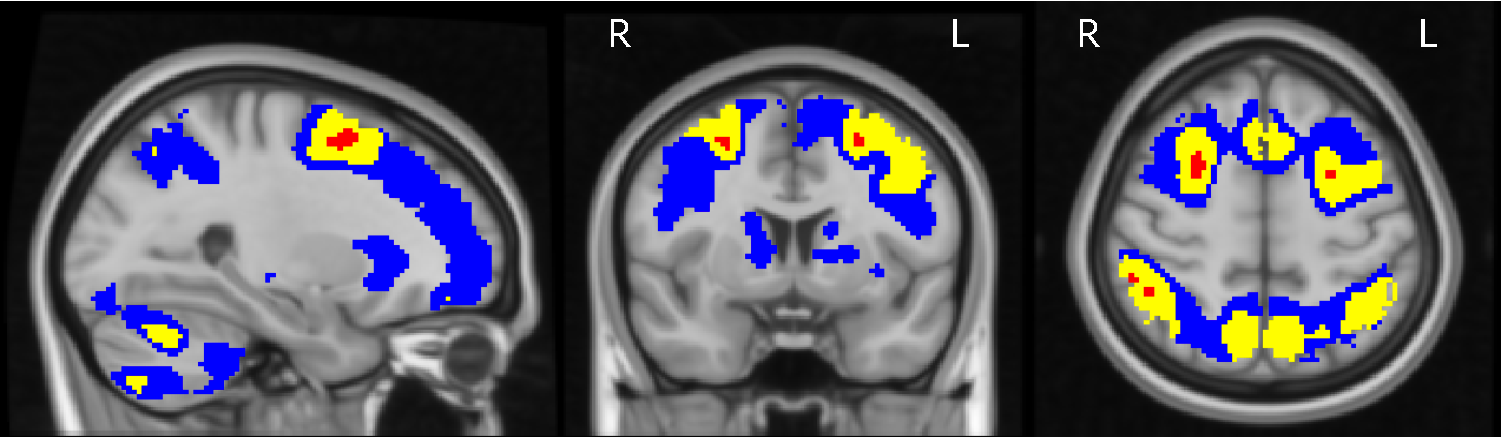
\includegraphics[height=45.5mm]{CIC_Fig1_Algorithm3_c08.pdf}\\
        1.2 Cohen's $d$ & 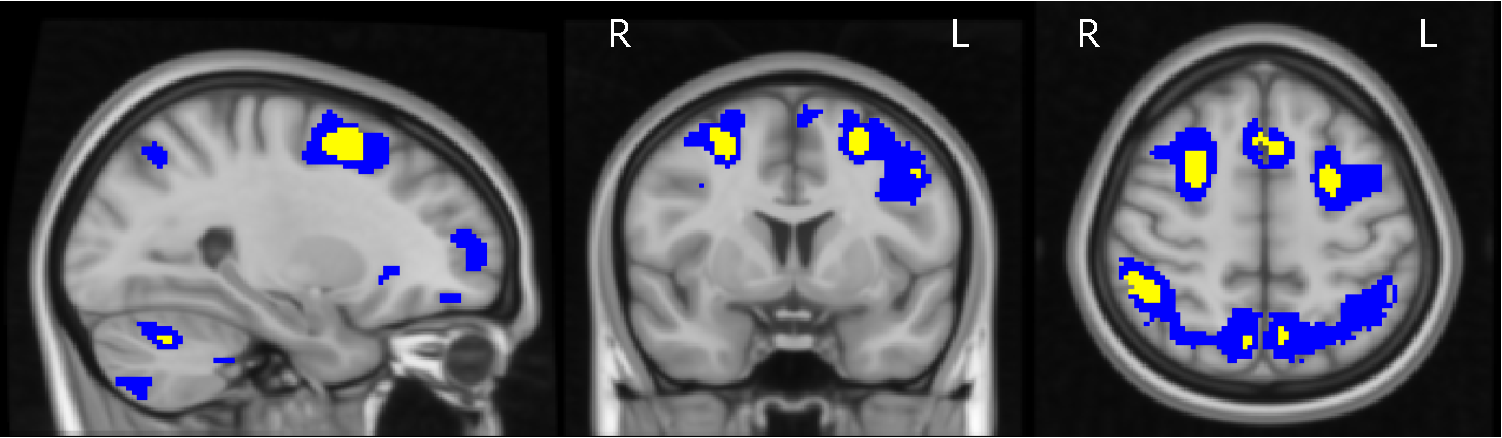
\includegraphics[height=45.5mm]{CIC_Fig1_Algorithm3_c12.pdf}\\
        \bottomrule
    \end{tabular}
\end{adjustbox}
    \captionof{figure}{Slices views of the Cohen's $d$ Confidence Sets obtained from applying Algorithm \ref{alg:three}.\ to the HCP working memory task data, using three Cohen's $d$ effect size thresholds, $c = 0.5, 0.8$ and $1.2$. The upper CS $\Ahatcp$ is displayed in red, and the lower CS $\Ahatcm$ in blue. Yellow voxels represent the point estimate set $\Ahatc$, the best guess from the data of voxels that have surpassed the Cohen's $d$ threshold. The red upper CS has localized regions in the frontal gyrus, paracingulate gyrus, angular gyrus, cerebellum and precuneus which we can assert with 95\% confidence have attained (at least) a 0.5 Cohen's $d$ effect size.}
    \label{fig:HCP_Algorithm_3}
\end{table}

\begin{table}[htbp]
\hspace*{-0.5cm}
\begin{adjustbox}{center}
\centering
    \begin{tabular}{cm{50mm}m{50mm}m{50mm}}
       \toprule
         Threshold $c$ & \hspace{1.4cm} Sagittal (X = 63) & \ \hspace{1.0cm} Coronal (Y = 130) & \hspace{0.9cm} Axial (Z = 124)\\
        \midrule
        0.5 Cohen's $d$ & 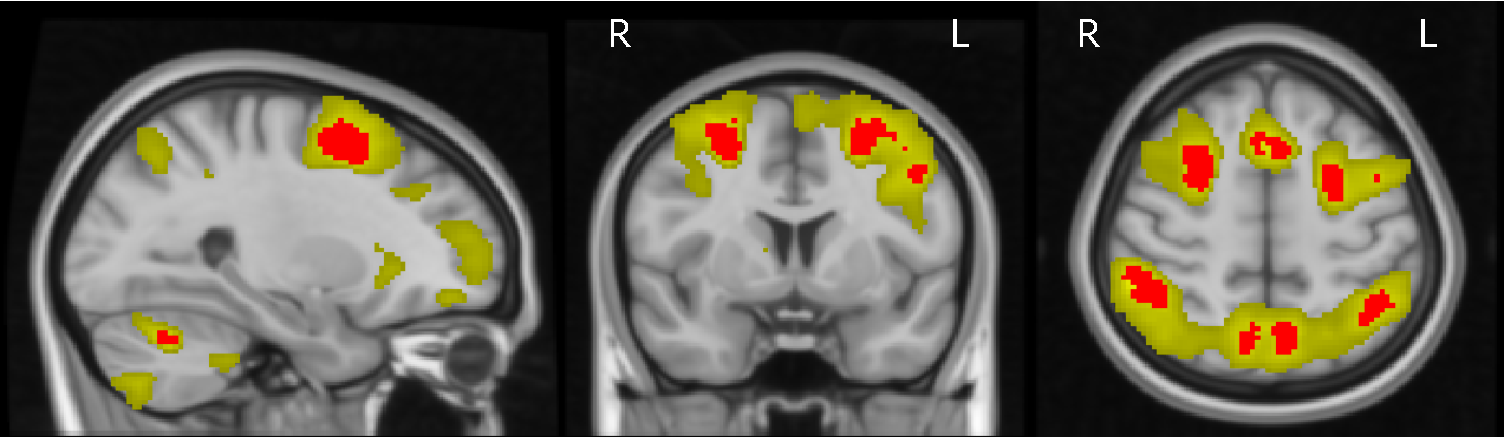
\includegraphics[height=45.5mm]{CIC_GLM_Algorithm3_c05.pdf}\\
        0.8 Cohen's $d$ & 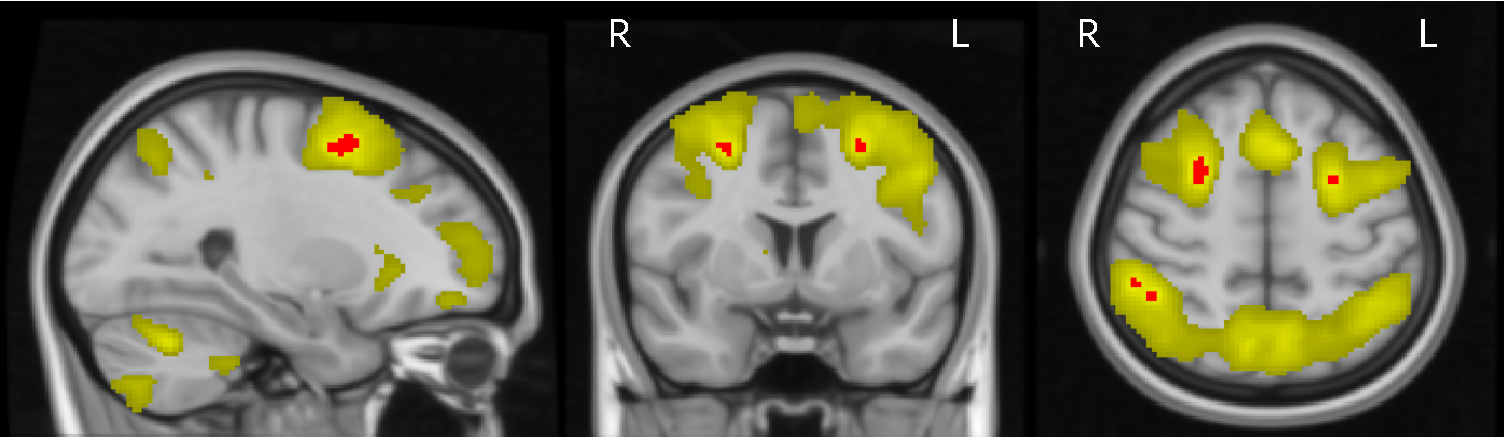
\includegraphics[height=45.5mm]{CIC_GLM_Algorithm3_c08.pdf}\\
        1.2 Cohen's $d$ & 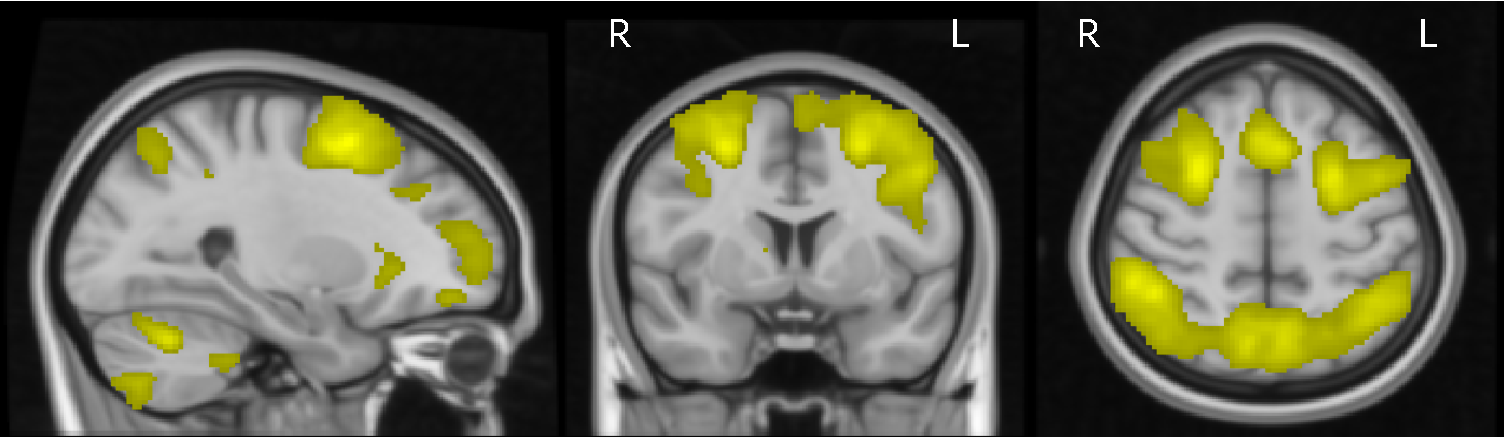
\includegraphics[height=45.5mm]{CIC_GLM_Algorithm3_c12.pdf}\\
        \bottomrule
    \end{tabular}
\end{adjustbox}
    \captionof{figure}{Comparing the upper Confidence Sets computed with Algorithm 3.\ on the HCP working memory task data (same slice views as Fig.\ \ref{fig:HCP_Algorithm_3}) with the thresholded $t$-statistic results obtained by applying a traditional group-level one-sample $t$-test, voxelwise $p < 0.05$ FWE correction (green-yellow voxels). While the thresholded statistic map contains a single cluster covering a sizable portion of the parietal lobe across both hemispheres (axial slices), the upper CSs have localized the precise areas of the precuneus and anglur gyrus where we can confidently declare a Cohen's $d$ effect size of at least 0.5. This demonstrates how the CSs can provide improved spatial specificity in determining regions where practically significant activation has occured.}
    \label{fig:HCP_Algorithm_3_vs_GLM}
\end{table}


\subsection{Comparison to Traditional Inference Procedures}

\section{Discussion}

\subsection{Limitations}

\section{Conclusion}
